\documentclass{article}


\newlength\tindent
\setlength{\tindent}{\parindent}
\setlength{\parindent}{0pt}
\renewcommand{\indent}{\hspace*{\tindent}}

\usepackage{amssymb} % For \mathbb
\usepackage{amsmath}
\usepackage{xcolor}
\usepackage{array} % for better column definitions
\usepackage{listings}
\usepackage{tcolorbox}
\usepackage{tikz}
\usetikzlibrary{matrix, positioning}
\newcommand{\negation}{${\phantom{0}}^\sim$}
\newcommand{\bul}[1]{\textcolor{blue}{\underline{#1}}}
\newcommand{\rul}[1]{\textcolor{red}{\underline{#1}}}
\newcommand{\sub}[1]{\vspace{10pt}\textbf{#1}}
\newcommand{\sbreak}{\vspace{10pt}}
\newcommand{\ssbreak}{\vspace{5pt}}
\usepackage{hyperref} % import the package

\lstset{
    language=Matlab,                  % Set the language
    frame=single,                     % Single frame around the code
    basicstyle=\small\ttfamily,      % Basic font style
    commentstyle=\color{green!50!black}, % Color for comments
    keywordstyle=\color{blue},       % Color for keywords
    stringstyle=\color{red},         % Color for strings
    xleftmargin=0in,
    xrightmargin=0in,
    tabsize=1,
    literate={'}{\textquotesingle}1
}

\title{MA1522 Notes}
\begin{document}

\section{Linear Systems}
\subsection{Linear Equations}
A \bul{linear} equation with n variables in \bul{standard form} is:
\begin{center}
    \begin{math}
        a_1x_1 + a_2x_2 + ... + a_nx_n = b
    \end{math}
\end{center}

It is \bul{homogeneous} if b = 0

\subsection{Linear Systems}
A \bul{system of linear equations/linear system} consists of n variables and m equations:

\[
\left\{
\begin{array}{lcl}
a_{11}x_1 + a_{12}x_2 + \cdots + a_{1n}x_n & = & b_1 \\
a_{21}x_1 + a_{22}x_2 + \cdots + a_{2n}x_n & = & b_2 \\
\vdots & & \vdots \\
a_{m1}x_1 + a_{m2}x_2 + \cdots + a_{mn}x_n & = & b_m \\
\end{array}
\right.
\]

\subsection{General Solution}
The \bul{general solution} of a linear system captures \textcolor{red}{all possible} solutions of the linear system.

When there are inf. many solutions, we can assign variables as parameters.

\vspace{10pt}

Example general solution


\[
\left( 
\begin{array}{cccc|c}
x_1 & x_2 & x_3 & x_4 & \\
\hline
1 & 0 & -2 & 0 & 3 \\
0 & 1 & 4 & 0 & -1 \\
0 & 0 & 0 & 1 & 2 \\
\end{array}
\right)
\]

Assigning the arbitrary variable \textit{t} to $x_3$, we have the general solution:


\begin{gather*}
    x_1 = 3 + 2t \\
    x_2 = -1 - 4t \\
    x_3 = t \\ 
    x_4 = 2
\end{gather*}

Note that you can work backwards from a general solution to get an augmented matrix in RREF.

\subsection{Inconsistency/No Solution}
A linear system that is \textit{inconsistent} has no solution. Otherwise, if it has at least one solution, it is \bul{consistent}.

\subsection{Augmented Matrices}
A linear system can be represented as an \bul{augmented matrix}. Its dimensions are m x n, where m is the number of rows and n is the number of columns.

\[
\left( 
\begin{array}{cccc|c}
    x_1 & x_2 & \cdots  & x_n & \\
    \hline
a_{11} & a_{12} & \cdots & a_{1n} & b_1 \\
a_{21} & a_{22} & \cdots & a_{2n} & b_2 \\
\vdots & \vdots & \ddots & \vdots & \vdots \\
a_{m1} & a_{m2} & \cdots & a_{mn} & b_m \\
\end{array}
\right)
\]
\textit{(Top row was added to show how each column in the matrix represents a variable in the system)}

\vspace{10pt}

\textbf{Matrix indexing}

The (a,b) entry of a matrix is the item in the $a^{th}$ row and $b^{th}$ column.

\subsubsection{Solving matrix equations}
If we want to find Ax = b, we are essentially finding a coefficient vector x such that the transformation x on A results in the vector b.

If A is invertible, we can also take: x = $A^{-1}b = x$

\subsection{Row-echelon form}
An augmented matrix is in \bul{row-echelon form(REF)} if

1. If \textcolor{orange}{zero rows} exist, they are at the bottom of the matrix

2. The \textcolor{orange}{leading entries are further to the right} as we move down the rows.

\vspace{10pt}

Example:

\[
\left( 
\begin{array}{cccc|c}
1 & 2 & 3 & 2 & 9 \\
0 & 1 & 4 & 2 & 5 \\
0 & 0 & 3 & 2 & 1 \\
\end{array}
\right)
\]

\[
\begin{array}{ccccc}
    & & & \hspace{10pt} \uparrow  & \\    
    & & & \hspace{10pt} \text{non-pivot}  & \\    
\end{array}
\]


A column containing a leading entry is called a \bul{pivot column}. Otherwise, it is a non-pivot column.

\subsection{Reduced Row-Echelon form}
The augmented matrix is in RREF if

3. The \textcolor{orange}{leading entries} are 1.

4. In each \textcolor{orange}{pivot column}, all entries \textcolor{red}{except} the leading entry is 0.

\vspace{10pt}

Example: 

\[
\left( 
\begin{array}{ccc|c}
1 & 0 & 0 & 9 \\
0 & 1 & 0 & 5 \\
0 & 0 & 1 & 1 \\
\end{array}
\right)
\]

\subsection{Elementary Row Operations}
There are 3 types of \bul{elementary row operations}:

\vspace{10pt}

1. Exchanging two rows, $R_i \leftrightarrow R_j$

2. Adding a scalar multiple of a row to another $R_i + cR_j, c\in \mathbb{R}$

3. Multiplying the row by a \textcolor{red}{nonzero} constant

\vspace{10pt}

Note that performing elementary row operations preserves the solutions of the matrix.

\vspace{10pt}

\textbf{Row Equivalence}

Two elementary matrices have the \textcolor{orange}{same solutions} if their augmented matrices are \bul{row equivalent}, that is, one can be obtained from the other by performing a set of \textcolor{orange}{elementary row operations}

\vspace{10pt}

\textbf{Reversing Row Operations}

Elementary row operations can be reversed.

\vspace{10pt}

1. The reverse of exchanging two rows $R_i \leftrightarrow R_j$ is \textcolor{orange}{itself}.

2. The reverse of adding a multiple of a row to another, \textcolor{orange}{$R_i + cR_j$}, is subtracting the multiple of that row: \textcolor{orange}{$R_i - cR_j$}.

3. The reverse of multiplying a row by a nonzero constant, \textcolor{orange}{$aR_j$}, is multiplying the reciprocal: \textcolor{orange}{$\frac{1}{a}R_j$}

\subsection{Row Reduction}
An algorithm to reduce rows is described below

\vspace{10pt}

\textbf{Gaussian Elimination}

1. Locate the leftmost column that does not consist entirely of zeroes.

2. \textcolor{orange}{Interchange} the top row with another row to bring a nonzero entry to the top of the column.


3. For each row below the top row, \textcolor{orange}{subtract} a suitable multiple of the top row so that the entry below becomes zero.

4. Now, cover the top row and start with step 1 again.


\vspace{10pt}

Step 1 \& 2: Locate non-zero then swap
\[
\left(
\begin{array}{ccc|c}
0 & 2 & 3 & 8 \\
4 & 2 & 2 & 7 \\
2 & 7 & 3 & 1 \\
\end{array}
\right)
\xrightarrow{\text{$R_2 \leftrightarrow R_1$}} 
\left(
\begin{array}{ccc|c}
4 & 2 & 2 & 8 \\
0 & 2 & 3 & 6 \\
2 & 7 & 3 & 1 \\
\end{array}
\right)
\]

\vspace{10pt}

Step 3: Subtract multiple to make bottom entries 0
\[
\left(
\begin{array}{ccc|c}
    4 & 2 & 2 & 8 \\
    0 & 2 & 3 & 6 \\
    2 & 7 & 3 & 1 \\
\end{array}
\right)
\xrightarrow{\text{$R_3 - \frac{1}{2}R_1$}} 
\left(
\begin{array}{ccc|c}
4 & 2 & 2 & 8 \\
0 & 2 & 3 & 6 \\
0 & 6 & 1 & -3 \\
\end{array}
\right)
\]

Step 4: Cover the top row and repeat steps 1-3
\[
\left(
\begin{array}{cc|c}
2 & 3 & 6 \\
6 & 1 & -3 \\
\end{array}
\right)
\]

\vspace{10pt}

\textbf{Gaussian-Jordan Elimination}

Jordan adds two key steps to get the full RREF. Not sure why Gauss didn't think of it.

5. Multiply a suitable constant to each row such that all \mbox{\textcolor{orange}{leading entries become 1}}

6. Beginning with the last nonzero row and working upward, add suitable multiples of each row to the rows above to make them \textcolor{orange}{zero}

\vspace{10pt}

Step 5: Make the leading entries 1

\[
\left(
\begin{array}{ccc|c}
4 & 2 & 2 & 8 \\ &&& \\
0 & 2 & 3 & 6 \\ &&& \\ 
0 & 0 & -8 & -3 \\
\end{array}
\right)
\xrightarrow{\frac{1}{4}R_1, \frac{1}{2}R_2, -\frac{1}{8}R_3} 
\left(
\begin{array}{ccc|c}
1 & \frac{1}{2} & \frac{1}{2} & 4 \\ &&& \\ 
0 & 1 & \frac{3}{2} & 3 \\ &&& \\ 
0 & 0 & 1 & \frac{3}{8} \\
\end{array}
\right)
\]

\vspace{10pt}

Step 6: Starting from the bottom, make the upper entries 0.

\[
\left(
\begin{array}{ccc|c}
    1 & \frac{1}{2} & \frac{1}{2} & 4 \\ &&& \\ 
    0 & 1 & \frac{3}{2} & 3 \\ &&& \\ 
    0 & 0 & 1 & \frac{3}{8} \\
\end{array}
\right)
\xrightarrow{R_2 - \frac{3}{2}R_3,\\ R_1 - \frac{1}{2}R_3} 
\left(
\begin{array}{ccc|c}
1 & \frac{1}{2} & 0 & \frac{61}{16} \\ &&& \\ 
0 & 1 & 0 & \frac{39}{16} \\ &&& \\ 
0 & 0 & 1 & \frac{3}{8} \\
\end{array}
\right)
\]

\vspace{2pt}

\textit{(I should have probably used nicer numbers, but the world isn't nice.)}

\vspace{10pt}

\begin{tcolorbox}[title=MATLAB tip, colback=blue!5, colframe=blue!80!black]
    Get the RREF of matrices through MATLAB using the following:
    \begin{lstlisting}
% Set formatting to rational for
% fractions if you want
format("Rational")
% define variables if you need to
syms a,b,c
% create the augmented matrix 
A = [0 2 3 8; 4 2 2 7; a 7 3 1;]
% call rref function
rref(A)
    \end{lstlisting}
\end{tcolorbox}

\vspace{10pt}

\textbf{A note on Gaussian-Jordan eliminations with variables}

If the matrix you're working with has unknown variables (such as \textcolor{orange}{\textit{a}}), try to firstly avoid multiplying the reciprocal, e.g. \textcolor{orange}{$\frac{1}{a}R_i$}. If you do do this, ensure to account for when $a=0$, where $\frac{1}{a}$ is \textcolor{red}{not well-defined}.

\section{Matrix Algebra}

\subsection{Types of Matrices}

\subsubsection{Vectors}
An n x 1 matrix is called a \bul{column vector}, and a 1 x n matrix is called a \bul{row vector}

\[
\begin{array}{c|c}
\text{Column Vector} & \text{Row Vector} \\ \\
\begin{pmatrix}
a_1 \\
a_2 \\
a_3 
\end{pmatrix}
& 
\begin{pmatrix}
b_1 & b_2 & b_3 
\end{pmatrix}
\end{array}
\]

\subsubsection{Zero Matrices}
Denoted $0_{m\times n}$, it is an m x n matrix with all entries equal to 0.

\begin{center}
    3 x 4 zero matrix
\end{center}
\[
\left(
\begin{array}{cccc}
    0 & 0 & 0 & 0\\  
    0 & 0 & 0 & 0\\  
    0 & 0 & 0 & 0\\
\end{array}
\right)
\]

\subsubsection{Diagonal Matrix}
A Matrix where all non-diagonals are 0.

\[
\begin{pmatrix}
d_1 & 0 & 0 \\
0 & d_2 & 0 \\
0 & 0 & d_3 
\end{pmatrix}
\]

$d_x$ can be any number, including 0.

\subsubsection{Scalar Matrix}
Similar to diagonal matrix, but all elements along the diagonal are \textcolor{red}{the same}.

\[
\begin{pmatrix}
c & 0 & 0 \\
0 & c & 0 \\
0 & 0 & c 
\end{pmatrix}
\]

c must be the same number across the diagonal.

\subsubsection{Identity Matrix}
All elements across the diagonal \textcolor{red}{must be 1}

\[
\begin{pmatrix}
1 & 0 & 0 \\
0 & 1 & 0 \\
0 & 0 & 1 
\end{pmatrix}
\]

\subsubsection{Upper Triangular Matrix}
Informally, a matrix that forms a triangle along the diagonal, upwards.

$a_{ij} = 0$ for all i $>$ j


\[
\begin{pmatrix}
a_{11} & a_{12} & a_{13} \\
0 & a_{22} & a_{23} \\
0 & 0 & a_{33} 
\end{pmatrix}
\]

\subsubsection{Strictly Upper Triangular Matrices}
Informally, a matrix that forms a triangle \textit{above} the diagonal.

$a_{ij} = 0$ for all i $\geq$ j

\[
\begin{pmatrix}
0 & a_{12} & a_{13} \\
0 & 0 & a_{23} \\
0 & 0 & 0 
\end{pmatrix}
\]

\subsubsection{Lower Triangular Matrix}
Informally, a matrix that forms a triangle along the diagonal, downwards.

$a_{ij} = 0$ for all i $<$ j

\[
\begin{pmatrix}
a_{11} & 0 & 0 \\
a_{21} & a_{22} & 0 \\
a_{31} & a_{32} & a_{33} 
\end{pmatrix}
\]


\subsubsection{Strictly Lower Triangular Matrix}
Informally, a matrix that forms a triangle \textit{below} the diagonal.

$a_{ij} = 0$ for all i $\leq$ j

\[
\begin{pmatrix}
0 & 0 & 0 \\
a_{21} & 0 & 0 \\
a_{31} & a_{32} & 0 
\end{pmatrix}
\]

\subsubsection{Notes on triangular matrices}
For any triangular matrix of the same type, strict or not, their sums and products are of the same type.

\subsubsection{Symmetric Matrices}
For any $i, j$, $A_{ij} = A_{ji}$. The diagonal can be any number.

\[
\begin{pmatrix}
a_{11} & \textcolor{red}{a_{12}} & \textcolor{blue}{a_{13}} \\
\textcolor{red}{a_{12}} & a_{22} & \textcolor{orange}{a_{23}} \\
\textcolor{blue}{a_{13}} & \textcolor{orange}{a_{23}} & a_{33} 
\end{pmatrix}
\]

Note that if $A$ is symmetric,then $A^2$ is symmetric
\subsection{Matrix Equality}
Two matrices are equal iff they are the \textcolor{red}{same size} and their \textcolor{red}{corresponding entries are equal.}

\subsection{Scalar Matrix Multiplication}
A scalar constant $\lambda$ can be multiplied to a matrix.

\[
\lambda \cdot
\begin{pmatrix}
a_{11} & a_{12} & a_{13} \\
a_{21} & a_{22} & a_{23} \\
a_{31} & a_{32} & a_{33}
\end{pmatrix}
=
\begin{pmatrix}
\lambda a_{11} & \lambda a_{12} & \lambda a_{13} \\
\lambda a_{21} & \lambda a_{22} & \lambda a_{23} \\
\lambda a_{31} & \lambda a_{32} & \lambda a_{33}
\end{pmatrix}
\]
\begin{center}
    Where $\lambda$ is any real number.
\end{center}

\subsection{Matrix Addition}
Matrices can be added to each other, but is only defined between matrices of the same size.

\[
\begin{pmatrix}
a_{11} & a_{12} & a_{13} \\
a_{21} & a_{22} & a_{23} \\
a_{31} & a_{32} & a_{33}
\end{pmatrix}
+
\begin{pmatrix}
b_{11} & b_{12} & b_{13} \\
b_{21} & b_{22} & b_{23} \\
b_{31} & b_{32} & b_{33}
\end{pmatrix}
=
\begin{pmatrix}
a_{11} + b_{11} & a_{12} + b_{12} & a_{13} + b_{13} \\
a_{21} + b_{21} & a_{22} + b_{22} & a_{23} + b_{23} \\
a_{31} + b_{31} & a_{32} + b_{32} & a_{33} + b_{33}
\end{pmatrix}
\]

\subsection{Properties of Matrix Addition and Scalar Multiplation}

\begin{enumerate}
    \item \bul{Commutative}: A + B = B + A
    \item \bul{Associative}: A + (B + C) = (A + B) + C
    \item \bul{Additive Identity}: $0_{m\times n}$ + A = A 
    \item \bul{Additive Inverse}: A + (-A) = $0_{m\times n}$
    \item \bul{Distributive Inverse} a(A+B) = $aA + aB$
    \item \bul{Scalar addition} a+b(A) = $aA + bA$
    \item \bul{Associative} (ab)A = $a(bA)$
    \item \bul{} if aA = $0_{m\times n}$, then either a = 0 or A = 0
\end{enumerate}

\subsection{Matrix Multiplication}
Symbolically, AB = $(a_{ij})_{m\times p}(b_{ij})_{p\times n} = (\sum^p_{k=1}a_{ik}b_{kj})_{m\times n}$. But what the hell does that mean?

\begin{enumerate}
    \item If $A_{m\times b}$, and $B_{p\times n}$, then the resultant matrix is $AB_{m\times n}$
    \item The $(\rul{i},\bul{j})^{th}$ item of AB is equal to:
    \item[] The summation of $A_{\rul{i}k} * B_{k\bul{j}}$ for all k in the enumeration of p (the common factor in the size of the matrix.)
\end{enumerate}

\subsubsection{An example of matrix multiplication}

\[
\begin{pmatrix}
a_{11} & a_{12} & a_{13} \\
a_{21} & a_{22} & a_{23} \\ 
a_{31} & a_{32} & a_{33}
\end{pmatrix}
\cdot
\begin{pmatrix}
b_{11} & b_{12} & b_{13} \\
b_{21} & b_{22} & b_{23} \\ 
b_{31} & b_{32} & b_{33}
\end{pmatrix}
\]

Then, the $(1,2)^{th}$ item of AB is:
\begin{center}
    $a_{11}*b_{12} + a_{12}*b_{22} + a_{13}*b_{32}$
\end{center}

\vspace{10pt}

\subsubsection{Visualizing matrix multiplication}

Localise the row and column vector. Looking at the example above, the $(\textcolor{red}{\underline{1}},\bul{2})^{th}$ item,

\vspace{10pt}

Take the \textcolor{red}{\underline{first row}} of the A matrix
\[
\begin{pmatrix}
    a_{11} & a_{12} & a_{13} \\
\end{pmatrix}
\]

\vspace{10pt}

Take the \bul{second column} of the B matrix
\[
\begin{pmatrix}
    b_{12} \\
    b_{22} \\ 
    b_{32}
\end{pmatrix}
\]

\vspace{10pt}

Rotate B anti-clockwise, overlay, and add.
\[
\begin{array}{ccc}
(a_{11} & a_{12} & a_{13}) \\
 * & * & *  \\
(b_{12} & b_{22} & b_{32}) \\
\parallel & \parallel & \parallel \\ 
a_{11}b_{12}\ +& a_{12}b_{22} &+\ a_{13}b_{32}
\end{array}
\]

\vspace{10pt}

Repeat for all other i, j. Suffer.

\subsubsection{Properties of Matrix Multiplication}
\begin{enumerate}
    \item Matrix multiplication is \textcolor{red}{non-commutative}. That is, AB not necessary equals BA.
    \begin{enumerate}
        \item If multiplying A to the left of B, AB, it is called \bul{pre-multiplying} A to B.
        \item If multiplying A to the right of B, BA, it is called \bul{post-multiplying} A to B.
    \end{enumerate}
    \item \bul{Associativity} (AB)C = A(BC)
    \item \bul{Left Distributive Law} A(B+C) = AB + AC
    \item \bul{Right Distributive Law} (A+B)C = AC + BC
    \item \bul{Commutes with scalar multiplication} cAB = (cA)B = A(cB)
    \item \bul{Multiplicative identity} For any m $\times$ n matrix A,\quad$I_{m}$A = A = A$I_{n}$
    \item \bul{Nonzero Zero Divisor} There exists A$\neq 0_{m \times p}$ and B$\neq 0_{p \times n}$ such that \mbox{AB = $0_{m \times n}$}
    \item \bul{Zero Matrix} For any m$\times$n matrix A, $A0_{n\times p}$ = $0_{m\times p}$ and $0_{p\times m}A=0_{p\times n}$
    \item \bul{Powers of Matrices} \textcolor{red}{(Only defined for \underline{square matrices!})}
    \begin{enumerate}
        \item $A^0$ = I
        \item $A^n = AA^{n-1}$ \textit{(Essentially, recursively multiply)}
    \end{enumerate}
\end{enumerate}

\subsection{Transposition of Matrices}
The \bul{transpose} of a $m \times n$ Matrix A, \bul{$A^T$} is the $n\times m$ matrix whose $(i,j)$ entry is the $(j,i)$ entry of A.

\[
\begin{pmatrix}
a_{11} & \textcolor{blue}{a_{12}} & \textcolor{blue}{a_{13}} \\
\textcolor{red}{a_{21}} & a_{22} & \textcolor{blue}{a_{23}} \\
\textcolor{red}{a_{31}} & \textcolor{red}{a_{32}} & a_{33} 
\end{pmatrix}
\rightarrow
\begin{pmatrix}
a_{11} & \textcolor{red}{a_{21}} & \textcolor{red}{a_{31}} \\
\textcolor{blue}{a_{12}} & a_{22} & \textcolor{red}{a_{32}} \\
\textcolor{blue}{a_{13}} & \textcolor{blue}{a_{23}} & a_{33} 
\end{pmatrix}
\]

\textit{(It doesn't visualize as nice in a non-square matrix but the idea holds)}

\begin{tcolorbox}[title=MATLAB tip, colback=blue!5, colframe=blue!80!black]
    Get the transpose of matrices through MATLAB using the following:
    \begin{lstlisting}
% define variables if you need to
syms a,b,c
% create the augmented matrix 
A = [0 2 3 8; 4 2 2 7; a 7 3 1;]
% transpose
transpose(A)
    \end{lstlisting}
\end{tcolorbox}

\subsubsection{Properties of Transposition}
\begin{enumerate}
    \item \bul{Transpose of a transpose} $({A^T})^T$ = A
    \item \bul{Transpose of a scalar} $(cA)^T = cA^T$
    \item \bul{Distributivity} $(A+B)^T = A^T + B^T$
    \item \bul{Distributivity under multiplication} $(AB)^T = B^TA^T$
\end{enumerate}

\subsection{Matrix \& Vector Equations}
We've seen how linear systems can be expressed as augmented matrices. With the properties of multiplication, we can also express them as a \bul{matrix equation}:

\[
\textcolor{blue}{
\begin{pmatrix}
a_{11} & a_{12} & \cdots & a_{1n} \\
a_{21} & a_{22} & \cdots & a_{2n} \\
\vdots & \vdots & \ddots & \vdots \\
a_{m1} & a_{m2} & \cdots & a_{mn}
\end{pmatrix}
}
\begin{pmatrix}
x_1 \\
x_2 \\
\vdots \\
x_n
\end{pmatrix}
=
\textcolor{orange}{
\begin{pmatrix}
b_1 \\
b_2 \\
\vdots \\
b_m
\end{pmatrix}
},
\quad \textcolor{blue}{A}x = \textcolor{orange}{b}
\]

\vspace{10pt}

or a \bul{vector equation}: 

\[
x_1
\textcolor{blue}{
\begin{pmatrix}
a_{11} \\
a_{21} \\
\vdots \\
a_{m1}
\end{pmatrix}
} + 
x_2
\textcolor{blue}{
\begin{pmatrix}
a_{12} \\
a_{22} \\
\vdots \\
a_{m2}
\end{pmatrix}
} + \cdots + 
x_n
\textcolor{blue}{
\begin{pmatrix}
a_{1n} \\
a_{2n} \\
\vdots \\
a_{mn}
\end{pmatrix}
} =
\textcolor{orange}{
\begin{pmatrix}
b_1 \\
b_2 \\
\vdots \\
b_m
\end{pmatrix}
}, \quad 
x_1 \textcolor{blue}{a_1} + x_2 \textcolor{blue}{a_2} + \cdots + x_n \textcolor{blue}{a_n} = \textcolor{orange}{b}
\]

In this notation, $a_i$ (the column vector) is called the \bul{coefficient vector} for the variable $x_i$

\vspace{10pt}

\textbf{Example}

\vspace{10pt}

The linear system:
\[
\begin{cases}
\textcolor{blue}{3}x + \textcolor{blue}{2}y - z = \textcolor{orange}{1} \\
x + \textcolor{blue}{2}y + z = \textcolor{orange}{3} \\
x + z = \textcolor{orange}{2}
\end{cases}
\]

can be written as a matrix equation:
\[
\textcolor{blue}{
\begin{pmatrix}
3 & 2 & -1 \\
1 & 2 & 1 \\
1 & 0 & 1
\end{pmatrix}
}
\begin{pmatrix}
x \\
y \\
z
\end{pmatrix}
=
\textcolor{orange}{
\begin{pmatrix}
1 \\
3 \\
2
\end{pmatrix}
}
\]

or a vector equation:
\[
x \textcolor{blue}{
\begin{pmatrix}
3 \\
1 \\
1
\end{pmatrix}
} + 
y \textcolor{blue}{
\begin{pmatrix}
2 \\
2 \\
0
\end{pmatrix}
} + 
z \textcolor{blue}{
\begin{pmatrix}
-1 \\
1 \\
1
\end{pmatrix}
} =
\textcolor{orange}{
\begin{pmatrix}
1 \\
3 \\
2
\end{pmatrix}
}
\]

\subsection{Homogeneous Linear Systems}
A homogeneous linear system, Ax = 0 is always \textcolor{red}{consistent}

\vspace{10pt}

The zero solution, where x = $0_{p\times n}$ is called the \bul{trivial solution}

\vspace{10pt}

The non-zero solution is called the \bul{nontrivial solution}. \textit{If} the homogeneous linear system has the nontrivial solution, it has infinitely many solutions.

\vspace{10pt}

If the trivial solution is a solution to the linear system, then it must be a homogeneous linear system.
\begin{center}
    $a_1x_1 + a_2x_2 + ... + a_nx_n = b$

    $0x_1 + 0x_2 + .... + 0x_n = 0$
\end{center}

In a homogeneous system, if there is \textbf{only} the trivial solution, then the columns are \bul{linearly independent}.

\subsubsection{Superposition Principle}
If we have the \underline{general solution} of a system Ax=0 ($v_h$), and we have any particular solution to \textbf{Ax=b} ($x_p$), then,
\begin{center}
    General Solution of Ax=b $\rightarrow$ x = $x_p$ + $v_h$
\end{center}

\subsubsection{Lemmas based on properties of Matrix Multiplication}

\vspace{10pt}

\textbf{Solutions of linear and homogeneous system}

If v is a particular solution to Ax = b, and u is a particular solution to the \bul{homogeneous} system Ax=0 (same coeff matrix A), then v + u is also a solution to Ax = b.

\vspace{10pt}

\bul{Proof}

By the distributive property of matrix multiplication,
\begin{center}
    \begin{math}
        A(v+u) = Av + Au = b + 0 = b
    \end{math}
\end{center}


\vspace{10pt}

\textbf{Solutions of a system minused by itself}

If $v_1$ and $v_2$ are solutions to the linear system Ax = b, then $v_1 - v_2$ is a solution to the \bul{homogeneous} linear system Ax = 0.

\bul{Proof}

Again, by the left distributive law,

\begin{center}
    \begin{math}
        A(v_1-v_2) = Av_1 - Av_2 = b - b = 0
    \end{math}
\end{center}

\subsection{Submatrices}
A $p\times q$ \bul{submatrix} of a $m\times n$ matrix A, is formed by taking a $p \times q$ block of the entries of A.

% commented out tikz for faster build times... TODO: uncomment when done

\[
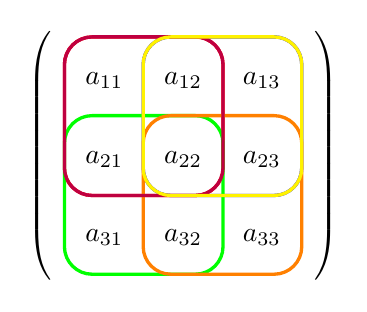
\begin{tikzpicture}
    % 3x3 matrix
    \matrix (m) [matrix of math nodes,left delimiter={(},right delimiter={)},nodes={minimum size=1cm, anchor=center, text height=1.5ex, text depth=0.25ex}] {
        a_{11} & a_{12} & a_{13} \\
        a_{21} & a_{22} & a_{23} \\
        a_{31} & a_{32} & a_{33} \\
    };

    % Box for first 2x2 submatrix (top-left)
    \draw[red,rounded corners=10pt,very thick] (m-1-1.north west) rectangle (m-2-2.south east);

    % Box for second 2x2 submatrix (top-middle)
    \draw[blue,rounded corners=10pt,very thick] (m-1-2.north west) rectangle (m-2-3.south east);

    % Box for third 2x2 submatrix (middle-left)
    \draw[green,rounded corners=10pt,very thick] (m-2-1.north west) rectangle (m-3-2.south east);

    % Box for fourth 2x2 submatrix (middle-right)
    \draw[orange,rounded corners=10pt,very thick] (m-2-2.north west) rectangle (m-3-3.south east);
    
    % Box for fifth 2x2 submatrix (bottom-left)
    \draw[purple,rounded corners=10pt,very thick] (m-1-1.north west) rectangle (m-2-2.south east);

    % Box for sixth 2x2 submatrix (bottom-right)
    \draw[yellow,rounded corners=10pt,very thick] (m-1-2.north west) rectangle (m-2-3.south east);
\end{tikzpicture}
\]
\textit{(Each color corresponds to a possible 2x2 submatrix)}

\subsection{Block Multiplication}
Using submatrices, we can define multiplication on a specific "block" of a matrix.

\vspace{10pt}

Formally, Let A be an $m \times p$ matrix and B a $p \times n$ matrix. Let $A_1$ be a $(m_2 - m_1 + 1) \times p$ submatrix of A obtained by taking
rows $m_1$ to $m_2$, and $b_1$ a $p \times (n_2 - n_1 + 1)$ submatrix of B obtained by taking columns $n_1$ to $n_2$. Then the product
$A_1B_1$ is a $(m_2 - m_1 + 1) \times (n_2 - n_1 + 1)$ submatrix of AB obtained by taking rows $m_1$ to $m_2$ and columns $n_1$ to $n_2$.

\vspace{10pt}

\textit{But what the hell does that mean?}

\subsubsection{Visualizing Block Matrix Multiplication}
Given a $3\times2$ matrix A, and a $2\times3$ matrix B, we know that the resultant matrix of AB is $3\times3$. How do we get the last two rows and columns (a 2x2 submatrix) of AB? Block matrix multiplication is how.

\vspace{10pt}

AB:

\[
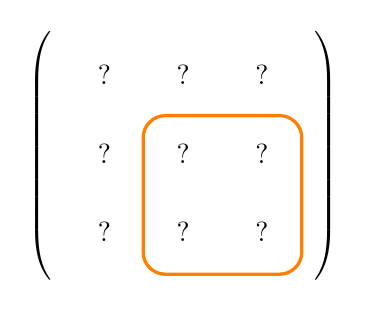
\begin{tikzpicture}
    % 3x3 matrix with question marks
    \matrix (m) [matrix of math nodes,left delimiter={(},right delimiter={)},nodes={minimum size=1cm, anchor=center, text height=1.5ex, text depth=0.25ex}] {
        ? & ? & ? \\
        ? & ? & ? \\
        ? & ? & ? \\
    };

    % Red box around the last two rows and columns (2x2 submatrix)
    \draw[orange,rounded corners=8pt,very thick] (m-2-2.north west) rectangle (m-3-3.south east);
\end{tikzpicture}
\]

We can take the \bul{second and third rows} of A, and the \rul{second and third columns} of B to find what the second and third rows and columns (a 2x2 submatrix) of AB is.

\vspace{10pt}

$A$:

\[
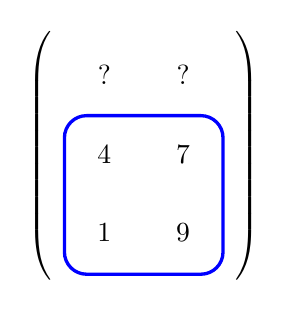
\begin{tikzpicture}
    % 3x2 matrix with random values and question marks
    \matrix (m) [matrix of math nodes,left delimiter={(},right delimiter={)},nodes={minimum size=1cm, anchor=center, text height=1.5ex, text depth=0.25ex}] {
        ? & ? \\
        4 & 7 \\
        1 & 9 \\
    };

    % Blue box around the second and third rows
    \draw[blue,rounded corners=8pt,very thick] (m-2-1.north west) rectangle (m-3-2.south east);
\end{tikzpicture}
\]

$B$:
\[
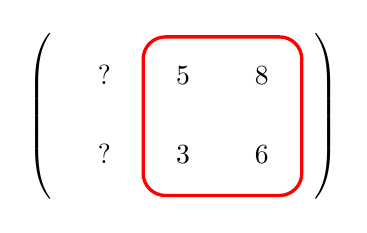
\begin{tikzpicture}
    % 2x3 matrix with random values and question marks
    \matrix (m) [matrix of math nodes,left delimiter={(},right delimiter={)},nodes={minimum size=1cm, anchor=center, text height=1.5ex, text depth=0.25ex}] {
        ? & 5 & 8 \\
        ? & 3 & 6 \\
    };

    % Red box around the second and third columns
    \draw[red,rounded corners=8pt,very thick] (m-1-2.north west) rectangle (m-2-3.south east);
\end{tikzpicture}
\]

$AB_{2\times 2}$:


\[
\textcolor{red}{
\begin{pmatrix}
5 & 8 \\
3 & 6 \\
\end{pmatrix}
}
\times
\textcolor{blue}{
\begin{pmatrix}
4 & 7 \\
1 & 9 \\
\end{pmatrix}
}
=
\textcolor{orange}{
\begin{pmatrix}
28 & 107 \\
18 & 75 \\
\end{pmatrix}
}
\]

Thus it can be seen that by localizing the correct submatrices, we can calculate the resultant submatrix.

\subsubsection{Using block multiplication to solve matrix equations}
\label{sec:ubmtsme}

If we have a coefficient matrix A, how do we find a $3\times3$ matrix X s.t. AX = b:
\[
\begin{pmatrix}
    4 & 7 & 3 \\
    8 & 2 & 3 \\
    1 & 9 & 3 \\
\end{pmatrix}
\times
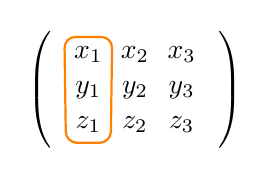
\begin{tikzpicture}[baseline=(m1.center)]
    \matrix (m1) [matrix of math nodes,left delimiter={(},right delimiter={)}]
    {
        x_1 & x_2 & x_3 \\
        y_1 & y_2 & y_3 \\
        z_1 & z_2 & z_3 \\
    };
    % Orange box around x_1, y_1, z_1
    \draw[orange, thick, rounded corners] 
        (m1-1-1.north west) -- (m1-3-1.south west) -- (m1-3-1.south east) -- (m1-1-1.north east) -- cycle;
\end{tikzpicture}
=
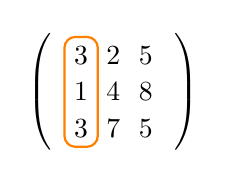
\begin{tikzpicture}[baseline=(m2.center)]
    \matrix (m2) [matrix of math nodes,left delimiter={(},right delimiter={)}]
    {
        3 & 2 & 5 \\
        1 & 4 & 8 \\
        3 & 7 & 5 \\
    };
    % Orange box around 3, 1, 3
    \draw[orange, thick, rounded corners] 
        (m2-1-1.north west) -- (m2-3-1.south west) -- (m2-3-1.south east) -- (m2-1-1.north east) -- cycle;
\end{tikzpicture}
\]


Because of block multiplication, we know we can take the $3\times3$ submatrix of A and a $3\times1$ submatrix of X to find out what the corresponding column vector (e.g. 
\(
\begin{pmatrix} 3 \\ 1 \\ 3 \end{pmatrix}
\)
) is.

We do this by arranging it in a augmented matrix, which we can stack to solve at once.
\[
\left(
\begin{array}{ccc|c|c|c}
    4 & 7 & 3 & 3 & 2 & 5 \\
    8 & 2 & 3 & 1 & 4 & 8 \\
    1 & 9 & 3 & 3 & 7 & 5 \\
\end{array}
\right)
\rightarrow
\left(
\begin{array}{ccc|c|c|c}
    1 & 0 & 0 & 1 & 0 & 2 \\
    0 & 1 & 0 & 3 & 9 & 7 \\
    0 & 0 & 1 & 4 & 4 & 5 \\
\end{array}
\right)
\]

Finding the RREF gives you the X matrix on the right hand side.

\subsubsection{Using block multiplication to find unknowns}
This is a natural extension from the previous example, but more complicated. Say we have matrixes A, B, and C s.t.

\[
\begin{array}{c}
    A \\
    \begin{pmatrix}
        x_{11} & x_{12} & x_{13} \\
        x_{21} & x_{22} & x_{23} \\
        x_{31} & x_{32} & x_{33}
    \end{pmatrix}
\end{array}
* 
\begin{array}{c}
    B \\
    \begin{pmatrix}
        1 & 21 & 3 & 4 \\
        2 & 21 & 5 & 6 \\
        7 & 21 & 8 & 9
    \end{pmatrix}
\end{array}
=
\begin{array}{c}
    C \\
    \begin{pmatrix}
        10 & \mathbf{?} & 12 & 13 \\
        14 & \mathbf{?} & 16 & 17 \\
        18 & \mathbf{?} & 20 & 21
    \end{pmatrix}
\end{array}
\]

We can use block multiplcation to create equations to solve for A. (e.g. ${x_{11} + 2x_{12} + 7x_{13} = 10}$). After getting A, we can multiply it to B to get the unknown column in C.

\subsection{Inverse of Matrices}
For a matrix to have an inverse, it must be such that $AA^{-1}\ =\ I\ =\ A^{-1}A$. From this, it can be easily seen that inverse for \rul{non-square} matrices is \rul{\textbf{not} well-defined!}.

\vspace{10pt}

So we define invertibility as such:

A \bul{$n\times n$} square matrix is \bul{invertible} if there exists a matrix \textbf{B} such that
\begin{center}
    $AB = I_n = BA$
\end{center}

Invertibility is an important rule on matrices, and given invertibility there are many statements that we can draw on the matrix.

\subsubsection{Computing an Inverse}
We can easily compute an inverse. Given that $AA^{-1}=I$, We can follow the same ideas as described in \hyperref[sec:ubmtsme]{2.11.2} to compute the inverse:
\[
\left( A \mid I \right) \xrightarrow{\text{RREF}} \left( I \mid A^{-1} \right)
\]

\begin{tcolorbox}[title=MATLAB tip, colback=blue!5, colframe=blue!80!black]
    Get the inverse of square matrices through MATLAB using the following:
    \begin{lstlisting}
% Set formatting to rational for
% fractions if you want
format("Rational")
% define variables if you need to
syms a,b,c
% create the augmented matrix 
A = [0 2 3; 4 2 2; a 7 3;]
% call inverse function
inv(A)
    \end{lstlisting}
\end{tcolorbox}


\subsubsection{Laws on Invertible Matrices}
All the following laws assume an $n\times n$ square matrix unless otherwise stated.


\sub{Law \#1: Inverse of 2$\times$2 Square Matrices}

A 2x2 square matrix A = 
\(
\begin{pmatrix}
    a & b \\
    c & d \\
\end{pmatrix}
\)
is invertible iff $ad - bc \neq 0$ and its inverse is given:

\vspace{10pt}
\begin{center}
    $A^{-1} = \frac{1}{ad - bc}$
    \(
    \begin{pmatrix}
        d & -b \\
        -c & a \\
    \end{pmatrix}
    \)
\end{center}

\sub{Law \#2: Cancellation Law of an invertible matrix}
\begin{enumerate}
    \item \bul{Left Cancellation}: if B and C are $n\times m$ matrices with $AB=AC$, then $B=C$
    \item \bul{Right Cancellation}: if B and C are $m\times n$ matrices with $AB=AC$, then $B=C$
\end{enumerate}

\sub{Law \#3: Consistency of Invertible Matrix and uniqueness of solution}

For any $n\times 1$ matrix b, $Ax = b$ has a unique solution.

\sub{Law \#4: Homogeneous Invertible System solution}

Given the invertible homogeneous linear system $Ax=0$, we can conclude that the trivial solution is the only solution.


\subsubsection{Properties of Inverses \& Equivalent Statements of Invertibility}
Given that A is invertible, (not every square matrix is invertible!),

\begin{enumerate}
    \item $(A^{-1})^{-1} = A$
    \item For any \rul{nonzero} real number a $\in \mathbb{R}$, aA is \bul{invertible} with inverse \mbox{$aA^{-1} = \frac{1}{a}A^{-1}$}
    \item $A^T$ is invertible with inverse $(A^{-1})^T$
    \item if B is an $n\times n$ \bul{invertible} matrix, then (AB) is \bul{invertible} with inverse $\mathbf{B^{-1}A^{-1}}$
    \begin{enumerate}
        \item Extending this law, if $(ABC)^{-1} = C^{-1}B^{-1}A^{-1}$
    \end{enumerate}
    \item A is invertible iff A is a product of elementary matrices
    \item A is invertible iff the RREF of A is the identity matrix
    \item A is invertible iff the \bul{homogeneous} system Ax=0 has only the trivial solution.
    \item A is invertible iff Ax=b has a \bul{unique} solution for all b.
    \item A is invertible iff it has a left inverse, i.e. BA = $I_n$
    \item A is invertible iff it has a right inverse, i.e. AB = $I_n$
    \item A is invertible iff \textcolor{red}{det(A) $\neq$ 0}
    \item A is invertible iff the columns/rows of A spans $\mathbb{R}^n$
    \item A is invertible iff the columns/rows of A are linearly independent
    \item A is invertible iff A has full rank
    \item A is invertible iff nullity(A) = 0
    \item A is invertible iff 0 is \rul{not} and eigenvalue of A.
    \item A is invertible iff the linear transformation T defined by A is \bul{injective} and \bul{surjective}
\end{enumerate}

\subsection{Elementary Matrices}
An $n\times n$ matrix n is called an \bul{elementary matrix} if it can be obtained from the identity matrix $I_{n}$ by performing a \textcolor{orange}{single elementary row operation}

\ssbreak

Performing row operations on any matrix is equivalent to premultiplying the corresponding elementary matrix. That is:

\begin{center}
    $A \overset{r}{\rightarrow} EA$
\end{center}
Where E is the elementary matrix corresponding to operation r.

\sbreak

Applying that repeatedly, we can define row equivalent matrices like so:
\begin{center}
    $A \overset{r_1}{\rightarrow} \overset{r_2}{\rightarrow} \cdots \overset{r_k}{\rightarrow} B$
    
    \ssbreak

    $B = E_k...E_2E_1A$
\end{center}

\sub{Manipulating Elementary Matrices}

If we know the RREF of A is I, that is, $A \overset{r_1}{\rightarrow} \overset{r_2}{\rightarrow} \cdots \overset{r_k}{\rightarrow} I$, then,
\begin{center}
    $I = E_k...E_1A$
\end{center}

We can make A the subject by premultiplying the inverse of each matrix onto I sequentially:
\begin{center}
    $A = E_1^{-1}...E_k^{-1}I = E_1^{-1}...E_k^{-1}$
\end{center}

Taking it further, we can derive $A^{-1}$ by taking the inverse of both sides and applying property \#4 and \#1 of inverses:
\begin{center}
    $A^{-1} = (E_1^{-1}...E_k^{-1})^{-1} = E_k...E_2E_1$
\end{center}

\subsubsection{Inverse of Elementary Matrices}
Every elementary matrix is \bul{invertible}, and corresponds to the \bul{reverse} of the row operation corresponding to E.

\begin{enumerate}
    \item 
    \[
    I_n \overset{R_i + cR_j}{\longrightarrow} E \quad \overset{R_i - cR_j}{\longrightarrow} I_n \quad \Rightarrow \quad E: R_i + cR_j, \quad E^{-1}: R_i - cR_j.
    \]
    
    \item 
    \[
    I_n \overset{R_i \leftrightarrow R_j}{\longrightarrow} E \quad \overset{R_i \leftrightarrow R_j}{\longrightarrow} I_n \quad \Rightarrow \quad E: R_i \leftrightarrow R_j, \quad E^{-1}: R_i \leftrightarrow R_j.
    \]
    
    \item 
    \[
    I_n \overset{cR_i}{\longrightarrow} E \quad \overset{\frac{1}{c}R_i}{\longrightarrow} I_n \quad \Rightarrow \quad E: cR_i, \quad E^{-1}: \frac{1}{c}R_i.
    \]
\end{enumerate}

\subsubsection{Elementary Matrices and Unit Lower Triangular Matrices}
\label{sec:emaultm}
See \hyperref[sec:ultm]{here} for definition on unit triangular matrix.

\sbreak

For a row operation $R_i + cR_j$ where \textbf{i $>$ j}, it's corresponding elementary matrix is a \bul{lower triangular matrix}

\ssbreak

$E^{-1}$ is also a unit triangular matrix.

\ssbreak

Then, if $E_1,E_2,E_3,....,E_k$ are row operations of the type $R_i + cR_j$ where $i>j$, then the $E_1E_2E_3..E_k$ and $E_1^{-1}E_2^{-1}E_3^{-1}..E_k^{-1}$ is a \bul{unit lower triangular matrix} as well.

\subsubsection{Determinant of Elementary Row Operations}
\textit{This section is repeated later but it's here for ease}
\[
\begin{array}{|c|c|}
\hline
\text{Transformation} & \text{Effect on Determinant} \\
\hline
A \xrightarrow{R_i + aR_j} B & \det(B) = \det(A) \\
A \xrightarrow{cR_i} B & \det(B) = c \det(A) \\
A \xrightarrow{R_i \leftrightarrow R_j} B & \det(B) = - \det(A) \\
\hline
\end{array}
\]

\subsection{LU Factorization}
LU factorization is the process of describing a matrix as a product of a \bul{unit lower triangular matrix} and a \bul{row-echelon} of A. We can write $A = LU$, where L is the lower triangular matrix, and U is a row-echelon form of A.


\[
A = \begin{pmatrix}
2 & 3 & 1 \\
4 & 7 & 7 \\
6 & 18 & 22
\end{pmatrix}
\]

The LU factorization of \( A \) is:

\[
A = LU
\]

where:

\[
L = \begin{pmatrix}
1 & 0 & 0 \\
2 & 1 & 0 \\
3 & 6 & 1
\end{pmatrix}
,\quad
U = \begin{pmatrix}
2 & 3 & 1 \\
0 & 1 & 5 \\
0 & 0 & 1
\end{pmatrix}
\]

\break

Note that not every matrix has a LU factorization. Additionally, A is \textbf{row-equivalent} to U.

\textit{Notice that LU factorization is just doing gaussian elimination on matrix. If there are situations in which you cannot form a unit lower triangular matrix when doing gaussian elimination (e.g. you have to swap a row), then you cannot LU factorize.}
\subsubsection{Unit Lower Triangular Matrices}
\label{sec:ultm}
Defined as a \textcolor{orange}{lower triangular} matrix with 1 as the diagonal entries:

\[
L = \begin{pmatrix}
1 & 0 & 0 & 0 \\
? & 1 & 0 & 0 \\
? & ? & 1 & 0 \\
? & ? & ? & 1
\end{pmatrix}
\]
\begin{center}
    Where ? is any real number.
\end{center}

\sub{A product of any unit triangular matrix is a unit triangular matrix too.}

\subsubsection{Algorithm to LU Factorize}
Using our knowledge on \hyperref[sec:emaultm]{elementary matrices and unit lower triangular matrices}, we compute a LU factorization for A.

\sbreak

Suppose 
\[
A \overset{r_1, r_2, \dots, r_k}{\longrightarrow} U
\]
where each row operation \(r_i\) is of the form \( R_i + cR_j \) for some $\mathbf{ i > j }$ and real number \( c \), and \( U \) is a row-echelon form of \( A \). Let \( E_i \) be the elementary matrix corresponding to \( r_i \), for \( i = 1, 2, \dots, k \). Then

\[
E_k \cdots E_2 E_1 A = U \quad \Rightarrow \quad A = E_1^{-1} E_2^{-1} \cdots E_k^{-1} U = LU
\]

where 
\[
L = E_1^{-1} E_2^{-1} \cdots E_k^{-1}.
\]
Then

\[
A = LU = 
\begin{pmatrix}
1 & 0 & 0 & 0 \\
* & 1 & 0 & 0 \\
* & * & 1 & 0 \\
* & * & * & 1
\end{pmatrix}
\begin{pmatrix}
* & * & * & * \\
0 & * & * & * \\
0 & 0 & * & * \\
0 & 0 & 0 & *
\end{pmatrix}
\]
is a LU factorization of \( A \).

\sbreak

To quickly compute the L matrix, for each row operation $r_x = R_i + c_xR_j$, simply put -$c_x$ in the (i,j) entry of L.

\begin{tcolorbox}[title=MATLAB tip, colback=blue!5, colframe=blue!80!black]
    Get the LU factorization using the following. Note that this is LU factorization \textit{without} pivoting. This function will not work if the diagonal coefficients are equal to 0.
    \begin{lstlisting}
% (credit to rayryeng on stackoverflow lol)
function [L, U] = lu_nopivot(A)

n = size(A, 1);
L = eye(n); 
for k = 1 : n
    L(k + 1 : n, k) = A(k + 1 : n, k) / A(k, k);
    for l = k + 1 : n
        A(l, :) = A(l, :) - L(l, k) * A(k, :);
    end
end
U = A;

end

% Define a matrix A
A = [2 3 1; 4 7 1;6 9 4]

% Call the function
[L,U] = lu_nopivot(A);
% If you're paranoid, verify L * U = a
L * U
    \end{lstlisting}
\end{tcolorbox}
\pagebreak
\subsubsection{Solving Matrix Equations using LU Factorizations}
Given a linear system Ax=b, and a LU factorization of A, the linear system can be re-written as $\mathbf{LUx=b}$.

\begin{enumerate}
    \item Let $Ux$ be an arbitrary variable y such that $\mathbf{Ly = b}$.
    \item Using archaic block multiplication knowledge detailed \hyperref[sec:ubmtsme]{here}, solve the system for \bul{y}.
    \item Now, we have a \textbf{Ux = y}. Apply step 2 but solve for x.
    \item Sacrifice a goat
\end{enumerate}

\subsection{Determinants}
The determinant is a value calculated from a matrix that lets us know if a matrix is invertible among other things.

\ssbreak


A matrix with detrminant 0 is called \rul{singular}.

\subsubsection{Determinant by Cofactor Expansion}
\[
\det(A) = \sum_{k=1}^{n} \textcolor{orange}{\underline{(-1)^{i+k}}} a_{ik} \det(A_{ik})
\]

\[
or
\]

\[
\det(A) = \sum_{k=1}^{n} \textcolor{orange}{\underline{(-1)^{j+k}}} a_{kj} \det(A_{kj})
\]

The formula essentially says that you can choose any 1 column or row and expand along that to calculate the determinant.

\sub{The sign of cofactor}

The orange underlined portion of the formula above is the \textcolor{orange}{\underline{sign of the cofactor}}, and can be visualised like so:

\[
\begin{pmatrix}
+ & - & + & \cdots \\
- & + & - & \cdots \\
+ & - & + & \cdots \\
\vdots & \vdots & \vdots & \ddots
\end{pmatrix}
\]

Any value along a \textit{diagonal} is \bul{positive}

\sub{Example of cofactor expansion}

Given a matrix:

\[
A = \begin{pmatrix}
a_{11} & a_{12} & a_{13} \\
a_{21} & a_{22} & a_{23} \\
a_{31} & a_{32} & a_{33}
\end{pmatrix}
\]

The determinant of \( A \) can be computed by cofactor expansion along the first row:

\[
\det(A) = a_{11} \begin{vmatrix} a_{22} & a_{23} \\ a_{32} & a_{33} \end{vmatrix}
- a_{12} \begin{vmatrix} a_{21} & a_{23} \\ a_{31} & a_{33} \end{vmatrix}
+ a_{13} \begin{vmatrix} a_{21} & a_{22} \\ a_{31} & a_{32} \end{vmatrix}
\]

This involves calculating the 2x2 determinants:

\[
\det(A) = a_{11}(a_{22}a_{33} - a_{23}a_{32}) 
- a_{12}(a_{21}a_{33} - a_{23}a_{31}) 
+ a_{13}(a_{21}a_{32} - a_{22}a_{31})
\]

\subsubsection{Determinant by Reduction}
Determinant by reduction is built on the fact that the determinant of a triangular matrix is the product of its diagonal entires.

\ssbreak

Knowing this, we can \bul{manipulate} any matrix to make it a triangular matrix and then multiply the diagonal entries to get the final determinant.

\sub{Determinant of Elementary Row Operations}
\[
\begin{array}{|c|c|}
\hline
\text{Transformation} & \text{Effect on Determinant} \\
\hline
A \xrightarrow{R_i + aR_j} B & \det(B) = \det(A) \\
A \xrightarrow{cR_i} B & \det(B) = c \det(A) \\
A \xrightarrow{R_i \leftrightarrow R_j} B & \det(B) = - \det(A) \\
\hline
\end{array}
\]

With the above if A and R are square matrices s.t. $A \xrightarrow{r_1} \xrightarrow{ r_2 } ... \xrightarrow{ r_k } R$,
\[
R = E_k...E_2E_1A
\]
Then,
\[
det(R) = det(E_k)...det(E_2)det(E_1)det(A)
\]

\subsubsection{Properties of Determinant}
\begin{enumerate}
    \item \bul{Invariant under transpose}: det(A) = det($A^T$)
    \item \bul{Determinant of Product}: Provided A and B are the same size, det(AB) = det(A)det(B)
    \begin{enumerate}
        \item \bul{Determinant of Squares}: det($A^2$) = det(A)det(A) = $\text{(det(A))}^2$
    \end{enumerate}
    \item \bul{Determinant of Inverse}: Provided A is invertible, det($A^{-1}$) = $det(A)^{-1}$
    \item \bul{Determinant of Scalar Multiplication}: det(cA) = $c^ndet(A)$, where n is the order of the matrix A
\end{enumerate}

\subsubsection{Some Determinants}
\begin{enumerate}
    \item Determinant of a $n\times n$ Identity Matrix: 1
    \item Determinant of a \textit{negative} Identity Matrix: $(-1)^{n}$
    \item Determinant of a scalar matrix: $c^n$ where c is the scalar
    \item Determinant of a \bul{upper triangular} matrix: Product of its diagonal
\end{enumerate}

\subsection{Adjoint}
Similar to transposition, the \bul{adjoint} of A is the $n\times n$ square matrix whose (i,j) entry is the (j,i) \bul{cofactor} of A.

\[
\begin{pmatrix}
a_{11} & \textcolor{blue}{a_{12}} & \textcolor{blue}{a_{13}} \\
\textcolor{red}{a_{21}} & a_{22} & \textcolor{blue}{a_{23}} \\
\textcolor{red}{a_{31}} & \textcolor{red}{a_{32}} & a_{33} 
\end{pmatrix}
\xrightarrow{cofactor}
\begin{pmatrix}
cf_{11} & \textcolor{blue}{cf_{12}} & \textcolor{blue}{cf_{13}} \\
\textcolor{red}{cf_{21}} & cf_{22} & \textcolor{blue}{cf_{23}} \\
\textcolor{red}{cf_{31}} & \textcolor{red}{cf_{32}} & cf_{33} 
\end{pmatrix}
\xrightarrow{transpose}
\begin{pmatrix}
    cf_{11} & \textcolor{red}{cf_{21}} & \textcolor{red}{cf_{31}} \\
    \textcolor{blue}{cf_{12}} & cf_{22} & \textcolor{red}{cf_{32}} \\
    \textcolor{blue}{cf_{13}} & \textcolor{blue}{cf_{23}} & cf_{33}
\end{pmatrix}
\]

\sbreak

\begin{tcolorbox}[title=MATLAB tip, colback=blue!5, colframe=blue!80!black]
    Get the adjoint of matrices through MATLAB using the following:
    \begin{lstlisting}
% Define a function to get cofactors
function C = cofactor(A)
    n = size(A, 1);  % Get the size of the matrix
    C = zeros(n);    % Initialize the cofactor matrix
    
    for i = 1:n
        for j = 1:n
            % Calculate the minor
            % by removing the ith row and jth column
            M = A;
            M(i, :) = [];    % Remove the ith row
            M(:, j) = [];    % Remove the jth column
            
            % Calculate the cofactor
            C(i, j) = ((-1)^(i + j)) * det(M);
        end
    end
end

% create the augmented matrix 
A = [0 2 3 8; 4 2 2 7; 7 7 3 1;]
% get cofactor then transpose
transpose(cofactor(A))
    \end{lstlisting}
\end{tcolorbox}

\subsubsection{Adjoint Formula}
If A is a square matrix and adj(A) its adjoint. Then,
\begin{center}
    $A(adj(A)) = det(A)I$
\end{center}

\sub{Determinant of a square adjoint}

As we have the square formula above, we can use that to calculate a determinant of an adjoint given det(A).
\begin{center}
    det(A(adj(A))) = det(det(A)I)
\end{center}
det(A) is a scalar value, so det(A)*I is some identity matrix of scalar det(A). Recall the determinant of a triangular matrix is the product of it's diagonal. So, rearranging the RHS,
\begin{center}
    det(det(A)I) = $\text{det(A)}^n$
\end{center}
Using known properties of determinants, we re-arrange the left hand side to:
\begin{center}
    det(a) * det(adj(A))
\end{center}

Finally, we have
\begin{center}
    det(adj(A)) = $\frac{\text{det(A)}^n}{det(A)} = \text{det(A)}^{n-1}$
\end{center}

\subsubsection{Adjoint Formula for inverse}
\begin{center}
    $A^{-1} = \frac{1}{det(A)}adj(A)$
\end{center}

\section{Euclidian Vector Spaces}
Recall the definitions of Vectors:

v = $\begin{pmatrix}
    v_1\\
    v_2\\
    \vdots\\
    v_n
\end{pmatrix}$

Each entry $v_i$ is also known as the i-th coordinate.

The Euclidian n-space, denoted as $\mathbb{R}^n$ is the collection of all n-vectors

\[
\mathbb{R}^n = \left\{
v = \begin{pmatrix}
v_1 \\
v_2 \\
\vdots \\
v_n
\end{pmatrix} \mid v_i \in \mathbb{R} \text{ for } i = 1, \dots, n
\right\}.
\]

\subsection{Vector Algebra}
\textit{Note that bolded letters refer to vectors, and non-bolds refer to scalars}

\begin{enumerate}
    \item The sum \textbf{u} + \textbf{v} is a vector in $\mathbb{R}^n$
    \item \bul{Commutative}: \textbf{u} + \textbf{v} = \textbf{v} + \textbf{u}
    \item \bul{Associative}: \textbf{u} + (\textbf{v} + \textbf{w}) = (\textbf{u} + \textbf{v}) + \textbf{w}
    \item \bul{Zero vector}: 0 + \textbf{u} = \textbf{u}
    \item \bul{Negative Vector}: \textbf{-u} is a vector s.t. \textbf{u} + \textbf{-u} = 0
    \item \bul{Scalar Multiple}: c\textbf{u} is a vector in $\mathbb{R}^n$
    \item \bul{Distributivity of Scalar}:
    \begin{enumerate}
        \item a(\textbf{u} + \textbf{v}) = a\textbf{u} + a\textbf{v}
        \item (a+b)\textbf{u} = a\textbf{u} + b\textbf{u}
    \end{enumerate}
    \item \bul{Associativity of scalar multiplication}: (ab)\textbf{u} = a(b\textbf{u})
    \item \bul{Zero result}: If a\textbf{u} = 0, then either a = 0 or \textbf{u} = 0
\end{enumerate}

\subsection{Abstract Vector Spaces}
An abstract vector space is a \textit{mathematical structure} that consists of a set of objects that are not necessarily vectors that satisfy axioms of vector space. These objects can be functions, polynomials, matrices or any kind of mathematical object. They just have to \textbf{behave like a vector space}. This allows us to define vector spaces for non-vector objects, and answer exam questions so we don't fail.

\textit{Note that a \textbf{real} vector space is a specific instance of abstract vector spaces where the scalars are real numbers. It's \rul{not} the opposite of an abstract vector space as it may seem.}

\sbreak

A set V equipped with addition and scalar multiplication is said to be a vector space over $\mathbb{R}$ if it satisfies the following axioms:

\begin{enumerate}
    \item \bul{Inclusion of Sum}: For any vectors \textbf{u} and \textbf{v} in V, the sum \textbf{u} + \textbf{v} $\in$ V
    \item \bul{Commutativity}: For any vectors \textbf{u}, \textbf{v} in V, \textbf{u} + \textbf{v} = \textbf{v} + \textbf{u}
    \item \bul{Associativity}: For any vectors \textbf{u}, \textbf{v}, \textbf{w} in V, \textbf{u} + (\textbf{v} + \textbf{w}) = (\textbf{u} + \textbf{v}) + \textbf{w}
    \item \bul{Zero Vector}: There is a vector \textbf{0} in V such that 0 + \textbf{v} = \textbf{v} for all vectors in V.
    \item \bul{Negativity}: For any vector \textbf{u} in V, there exists a vector \textbf{-u} in V s.t. \textbf{u} + \textbf{-u} = 0
    \item \bul{Scaling}: For any scalar a in $\mathbb{R}$ and vector \textbf{u} in V, a\textbf{u} is a vector in V.
    \item \bul{Distributivity}: 
    \begin{enumerate}
        \item a(\textbf{u} + \textbf{v}) = a\textbf{u} + a\textbf{v}
        \item (a+b)\textbf{u} = a\textbf{u} + b\textbf{u}
    \end{enumerate}
    \item \bul{Associativity of scalar multiplication}: For any scalars a, b $\in \mathbb{R}$ and vector \textbf{u} in V, a(b\textbf{u}) = (ab)\textbf{u}
    \item \bul{Identity}: For any vector \textbf{u} in V, 1\textbf{u} = \textbf{u}
\end{enumerate}

\subsection{Multiplying Vectors (Dot Product)}
We can multiply two $n\times1$ vectors \textbf{u} and \textbf{v} (\textbf{u}$\cdot$\textbf{v}) by taking the transpose ($\mathbf{u}^T$) of the left vector multiplied by the right vector.

Doing this, the result is:
\begin{center}
    $u_1v_1 + u_2v_2 + ... + u_nv_n$
\end{center}
or symbolically, 
\begin{center}
    $\sum^n_{i=1}u_iv_i$
\end{center}

\subsection{Distance length of vector}
We can get a length of a vector $\begin{pmatrix}
    x\\
    y\\
\end{pmatrix}$ in $\mathbb{R}^2$ by using the pythagorean theorum.

\begin{center}
    $Distance = \sqrt{x^2+y^2}$
\end{center}

\sbreak

Similarly, for a vector $\begin{pmatrix}
    x \\
    y \\
    z\\
\end{pmatrix}$ in $\mathbb{R}^3$, we can compute:

\begin{center}
    $Distance = \sqrt{(\sqrt{x^2+y^2})^2 + z^2} = \sqrt{x^2+y^2+z^2}$
\end{center}

\subsection{Norm of a vector}
Using the pattern observed in finding a distance of a vector in $\mathbb{R}^2$ and $\mathbb{R}^3$, we can find a distance of \underline{any} vector through the following:

\begin{center}
    $\Vert u \Vert = \sqrt{u\cdot u} = \sqrt{u_1^2u_2^2+...+u_n^2}$
\end{center}

We call this the \bul{norm} of a vector.

\subsection{Properties involving the inner product and the norm}
Let \textbf{u} and \textbf{v} be vectors in $\mathbb{R}^n$ and a, b, c be some scalars

\begin{enumerate}
    \item \bul{Symmetric} \textbf{u} $\cdot$ \textbf{v} = \textbf{v} $\cdot$ \textbf{u}
    \item \bul{Scalar Multiplication}: c\textbf{u}$\cdot$\textbf{v} = (c\textbf{u})$\cdot$\textbf{v} = \textbf{u}$\cdot$(c\textbf{v})
    \item \bul{Distribution}: \textbf{u} $\cdot$ (a\textbf{v} + b\textbf{w}) = a\textbf{u}$\cdot$\textbf{v} + b\textbf{u}$\cdot$\textbf{w}
    \item \bul{Positive Definite}: \textbf{u}$\cdot$\textbf{u}$\geq$0 if and only if \textbf{u} = 0
    \item \bul{Norm of scalar multiples}: $\Vert c\textbf{u}\Vert = \mid c \mid \times \Vert \textbf{u} \Vert$
\end{enumerate}

\subsection{Unit Vectors}
A vector \textbf{u} is a \bul{unit vector} if its norm is 1.

\subsubsection{Normalizing}

We can \bul{normalize} a vector by multiplying it by the reciprocal of its norm.
\begin{center}
    Unit vector of \textbf{u} = $\textbf{u} \cdot \frac{1}{\Vert \textbf{u} \Vert}$
\end{center}

\subsubsection{Distance between vectors}
The distance between two vectors is the \bul{norm of their difference}:

\begin{center}
    distance between \textbf{u} and \textbf{v} = $\Vert \textbf{u} - \textbf{v} \Vert$
\end{center}

Plugging this into the formula for norms,

\begin{center}
    $\Vert \textbf{u} - \textbf{v} \Vert = \sqrt{(x_1 - x_2)^2 + (y_1 - y_2)^2 + ... + (z_1 - z_2)^2}$
\end{center}where $x_1 - z_1$ are coefficients in \textbf{u} and $x_2 - z_2$ are coefficients in \textbf{v}

\subsection{Angle between vectors}

While we're at this, we can also get the angle between two vectors \textbf{u} and \textbf{v} like so:

\begin{center}
    $\theta = \cos^{-1}(\frac{\textbf{u}\cdot\textbf{v}}{\Vert \textbf{u} \Vert \Vert \textbf{v} \Vert})$
\end{center}

\subsection{Linear Combinations}

Let \( \mathbf{u}_1, \mathbf{u}_2, \dots, \mathbf{u}_k \) be vectors in \( \mathbb{R}^n \). A linear combination of the vectors \( \mathbf{u}_1, \mathbf{u}_2, \dots, \mathbf{u}_k \) is
\[
c_1 \mathbf{u}_1 + c_2 \mathbf{u}_2 + \cdots + c_k \mathbf{u}_k,
\]
for some \( c_1, c_2, \dots, c_k \in \mathbb{R} \). The scalars \( c_1, c_2, \dots, c_k \) are called coefficients.

\subsection{Linear Spans}
The \bul{span} of a set of vectors is the subset of $\mathbb{R}^n$ containing \bul{all the linear combinations} of the vectors.

\sbreak

Informally put, it's the subspace/set of points that the vectors can "reach"

\subsubsection{Valid Spans}
A set S = \{$u_1, ..., u_k$\} is a valid span of the Euclidean n space if and only if $(u_1 u_2 ... u_k | v)$  is consistent for every $v \in \mathbb{R}^n$, that is, it has no zero rows.

\subsubsection{Checking if a vector falls in a span}
To check if a vector falls in a span, it is simply checking if the vector is a \bul{linear combination} of the set of vectors.

\sbreak


\begin{enumerate}
    \item Let S = $\{ \textbf{u}_1, \textbf{u}_2, ..., \textbf{u}_k \}$ be a set of vectors in $\mathbb{R}^n$
    \item Form the $n\times k$ matrix A = ($\textbf{u}_1\ \textbf{u}_2\ ...\ \textbf{u}_k$)
    \item Set up the equation Ax = v, where v is the vector that is being checked
    \item If the system is consistent, the vector is in the span of the vectors. The solutions to the system are the coefficients to the linear combination.
\end{enumerate}

\subsubsection{Example of checking for inclusion in span}
We want to check if \( \mathbf{v} = \begin{pmatrix} 7 \\ 5 \end{pmatrix} \) is in the span of \( \mathbf{u}_1 = \begin{pmatrix} 1 \\ 2 \end{pmatrix} \) and \( \mathbf{u}_2 = \begin{pmatrix} 3 \\ 1 \end{pmatrix} \).

We form an augmented matrix:
\[
\left(
\begin{array}{cc|c}
1 & 3 & 7 \\
2 & 1 & 5
\end{array}
\right)
\]

Perform row operations to find the RREF.
\[
\begin{pmatrix}
1 & 0 & \frac{8}{5} \\
0 & 1 & \frac{9}{5}
\end{pmatrix}.
\]

From this, we can see that V can be expressed as a linear combination of $u_1$ and $u_2$ like so:
\[
\mathbf{v} = \frac{8}{5} \mathbf{u}_1 + \frac{9}{5} \mathbf{u}_2.
\]

\subsubsection{Standard Basis}
A set of n vectors $\{ u_1, u_2, ... u_n \}$ is called a \bul{standard basis} if it spans the whole of $\mathbb{R}^n$

\sbreak

A set of vectors will be a standard basis if it's \bul{linearly independent}. We can check this by reducing the matrix A = $(u_1 u_2 ... u_n)$ and seeing if there are any non-pivot columns. If there are \rul{no non-pivot columns}, the vectors are linearly independent and span $\mathbb{R}^n$.

\subsubsection{Properties of Linear Spans}
\begin{enumerate}
    \item The \bul{zero vector} is in the span.
    \item The span is \bul{closed under scalar multiplication}. Any vector \textbf{u} in span(S) and scalar a, the vector a\textbf{u} is a vector in span(S).
    \item The span is \bul{closed under addition}. For any vectors \textbf{u} and \textbf{v} in span(S), their sum \textbf{u + v} is a vector in span(S)
    \item Condensing (2) and (3), the span is \bul{closed under linear combination}.
\end{enumerate}

\subsubsection{Subsets of Spans (Span relations)}
\label{sec:sossr}
To check if \( \text{span}(S) = \text{span}(T) \), we check that:
\begin{itemize}
    \item \( \text{span}(S) \subseteq \text{span}(T) \), that is, 
    \[
    \left(
    \begin{array}{c|c}
        T & S
    \end{array}
    \right)
    =
    \left(
    \begin{array}{cccc|c|c|c|c}
    \mathbf{v}_1 & \mathbf{v}_2 & \cdots & \mathbf{v}_m & \mathbf{u}_1 & \mathbf{u}_2 & \cdots & \mathbf{u}_k
    \end{array}
    \right)
    \]
    is \bul{consistent}.
    \item \( \text{span}(T) \subseteq \text{span}(S) \), that is,
    \[
    \left(
    \begin{array}{c|c}
        S & T
    \end{array}
    \right)
    =
    \left(
    \begin{array}{cccc|c|c|c|c}
    \mathbf{u}_1 & \mathbf{u}_2 & \cdots & \mathbf{u}_k & \mathbf{v}_1 & \mathbf{v}_2 & \cdots & \mathbf{v}_m
    \end{array}
    \right)
    \]
    is \bul{consistent}.
\end{itemize}

\sub{Example}

Let \( S = \left\{ \begin{pmatrix} 1 \\ 1 \\ 1 \end{pmatrix}, \begin{pmatrix} 2 \\ 3 \\ 2 \end{pmatrix} \right\} \)
and \( T = \left\{ \begin{pmatrix} 1 \\ 1 \\ 1 \end{pmatrix}, \begin{pmatrix} 1 \\ -1 \\ 0 \end{pmatrix}, \begin{pmatrix} 1 \\ 2 \\ 1 \end{pmatrix} \right\} \).

\sbreak

\textbf{To check if \( \text{span}(S) \subseteq \text{span}(T) \),} 
\[
\left(
\begin{array}{ccc|c|c|c}
1 & 1 & 1 & 1 & 1 & 2 \\
1 & -1 & 1 & 2 & 3 & 3 \\
1 & 1 & 1 & 1 & 1 & 2
\end{array}
\right)
\xrightarrow{RREF}
\left(
\begin{array}{ccc|c|c|c}
1 & 0 & 0 & 1 & 0 & 1 \\
0 & 1 & 0 & 0 & 0 & 0 \\
0 & 0 & 1 & 0 & 1 & 1
\end{array}
\right)
\]
\begin{center}
    This is \bul{consistent}
\end{center}

\sbreak

\textbf{To check if \( \text{span}(T) \subseteq \text{span}(S) \),}
\[
\left(
\begin{array}{ccc|c|c|c}
1 & 1 & 2 & 1 & 1 & 1 \\
1 & 2 & 3 & 1 & -1 & 2 \\
1 & 1 & 2 & 1 & 0 & 1
\end{array}
\right)
\xrightarrow{RREF}
\left(
\begin{array}{ccc|c|c|c}
1 & 0 & 1 & 0 & 1 & 0 \\
0 & 1 & 0 & 0 & 0 & 1 \\
0 & 0 & 0 & 0 & \textcolor{red}{1} & 0
\end{array}
\right)
\]
\begin{center}
    This is \rul{not consistent}
\end{center}

\sbreak


This shows that \( \text{span}(T) \not\subseteq \text{span}(S) \). In particular, 
$
\begin{pmatrix} 
1 \\ -1 \\ 0 
\end{pmatrix}
\notin \text{span}(S).
$

Span(S) $\subseteq$ span(T)


\subsection{Solution sets of a linear system}
The \bul{set} of solutions to a linear system Ax = b is a subset in $\mathbb{R}^n$. We can express the set in two ways:

\sub{\underline{Implicit} Expression of set of solutions}
\begin{center}
    V = \{ $u \in \mathbb{R}^n \mid \textbf{Au=b}$ \}

    \sbreak

    writing it out a little more verbosely,

    \sbreak

    V = $\left\{\begin{array}{c|c}
        \begin{pmatrix}
            u_1 \\
            u_2 \\
            \vdots \\
            u_n
        \end{pmatrix} & A\begin{pmatrix}
            u_1 \\
            u_2 \\
            \vdots \\
            u_n
        \end{pmatrix}
    \end{array}=b\right\}$
\end{center}

\sub{\underline{Explicit} Expression of set of solutions}
\begin{center}
$V = \{\bul{\mathbf{u} + s_1 \mathbf{v}_1 + s_2 \mathbf{v}_2 + \cdots + s_k \mathbf{v}_k} \mid s_1, s_2, \dots, s_k \in \mathbb{R}\}$

\sbreak

Where the \bul{blue section} is the \textcolor{orange}{general solution}
\end{center}


\subsubsection{Example: Writing out solution sets}
\label{sec:ewoss}
Considering this linear system:
\begin{align*}
    3x + 2y - z &= 0 \\
    y - z &= 0 
\end{align*}

We write the solution set \underline{implicitly} as:

\[
\left\{
\begin{array}{c|c}
    \begin{pmatrix}
        x \\ y \\ z
    \end{pmatrix} 
    &
    3x+2y-z=1,\ y-z=0
\end{array}
\right\}
\]

\sbreak

To write it out \underline{explicitly}, we must first get the general solution. Do this intuitively, or use an augmented matrix:

\[
\text{Augmented matrix:} \quad 
\begin{pmatrix}
3 & 2 & -1 & | & 1 \\
0 & 1 & -1 & | & 0
\end{pmatrix}
\]

\[
\text{RREF:} \quad 
\begin{pmatrix}
1 & 0 & \frac{1}{3} & | & \frac{1}{3} \\
0 & 1 & -1 & | & 0
\end{pmatrix}
\]

\textbf{\textcolor{red}{NOTE:}} that when you are writing the solution space out explicitly, you are finding the nullspace of the RREF.


From this, we can see that the general solution is:

$x = \frac{1}{3}(1-s),\ y=z=s,\ s\in\mathbb{R}$

From the general solution, we write the solution set \underline{explicitly} as:

\[
\left\{
\begin{array}{c|c}
    \begin{pmatrix}
        \frac{1}{3} \\ 0 \\ 0
    \end{pmatrix} + s 
    \begin{pmatrix}
        -\frac{1}{3} \\ 1 \\ 1
    \end{pmatrix}
    &
    s \in \mathbb{R}
\end{array}
\right\}
\]

\subsubsection{Spans of Solution Sets}
Writing out a solution set explicitly, we can easily see that a solution set spans a certain space itself. From the example above, the solution set is the span:
\begin{center}
    Span $\left\{\left(\begin{array}{c}
        -\frac{1}{3} \\ 1 \\ 1
    \end{array}\right)\right\} + \begin{pmatrix}
        \frac{1}{3} \\ 0 \\ 0
    \end{pmatrix}$
\end{center}
This is because of the free parameter s, which is any real number. So the amount of \bul{dimensions} that a \bul{solution set} spans is closely linked to the amount of \rul{non-pivot columns} in the solution. (\textit{this is an intuition that will help later})

\sbreak

We can also call this a subspace if it fulfils certain criteria.

\subsection{Subspaces}
Subset V of the Euclidean n-space is a vector space if it satisfies these 3 axioms:

\begin{enumerate}
    \item V contains the zero vector
    \item V is \bul{closed under scalar multiplication}. For any vector \textbf{u} in V and scalar a, the vector a\textbf{u} is in V.
    \item V is \bul{closed under addition}. For any \textbf{u}, \textbf{v} in V, the sum \textbf{u+v} is in V.
\end{enumerate}

\subsubsection{Homogeneous Linear Systems and Subspaces}
It turns out that for a linear system \textbf{Ax=b}, for its solution set \break V= \{ \textbf{u} $\mid$ Au = b\} to be a subspace, the system \rul{must be} \bul{homogeneous}. That is, Au = 0.

The solution set to a homogeneous system is called a \bul{solution space}.

\subsubsection{Subspaces under union}
For 2 subspaces V and W of arbitrary Euclidian space $\mathbb{R}^n$,

$V \cup W$ is a subspace \textbf{only if}
\begin{center}
    $V \subseteq W$ or $W \subseteq V$
\end{center}
This is because if they are not subsets of each other, then there exists some vector u$\in V$ (resp. W) such that v$\notin W$ (resp. V). This means that closure under addition \rul{is not guaranteed}

\sbreak

Geometrically, unioning subspaces represents the vectors that belong to V and W, but not their linear combinations.

\sub{Basis for combined subspace}
If B and C are bases for V and W, then $B \cup C$ is a basis for $V + W$, after removing dependent columns. $B + C$ is not the basis, because adding the columns together might introduce dependency.

\subsubsection{Subspaces under addition}
Two subspaces V and W are \textbf{always} subspaces under addition.
\begin{enumerate}
    \item V+W contains the zero vector; 0+0 = 0
    \item V+W is closed under scalar multiplication. (v + w) * 3 = (3v + 3w). Since V and W are closed under scalar multiplication itself, this holds
    \item V+W is closed under scalar addition. (3v + 3w) + (21v + 32w) = (24v + 35w). Same as above.
\end{enumerate}
Geometrically, adding subspace represents a subspace that spans all the vectors and linear combinations in V and W.

\subsubsection{Subspaces under Intersection}
Two subspaces V and W are \textbf{always} subspaces under Intersection
\begin{enumerate}
    \item $V \cap W$ contain the zero vector.
    \item $V \cap W$ is closed under addition: $x\in V\cap W \rightarrow (x \in V ) \cap (x \in W)$. Thus, addition is defined.
    \item $V \cap W$ is closed under scalar multiplication.
\end{enumerate}

Geometrically, intersecting two subspaces are the vectors contained in both bases.

\sub{Finding subspace of intersections}
You are essentially finding a subspace s.t. if V = \{$v_1, v_2, v_3$\} and W = \{$w_1, w_2, w_3$\}
\begin{center}
    $x \in V \cap W \rightarrow c_1v_1 + c_2v_2 + c_3v_3 = k_1w_2 + k_2w_2 + k_3w_3 = x$
\end{center}
Simply create an augmented matrix (V$|$W), then reduce

\subsubsection{Describing subsets using linear equations}
If you have a matrix U, and you want to describe U using some linear equation $ax_1 + bx_2 + ... + cx_n$, take transpose of U, RREF, and the general solution will describe a linear equation of that form.

\subsection{Linear Independence}
A set of vectors $\{u_1, u_2, ..., u_k\}$ are \bul{linearly independent} if and only if the only constants fulfilling the equation
\begin{center}
    $c_1u_1 + c_2u_2 + ... c_ku_k = 0$
\end{center}
are 0. That is to say, each vector contributes a unique value in a dimension (informally). If there exists some constant such that the equation is true, the set is \rul{linearly dependent}
Note: Any set containing the 0 vector is \rul{linearly dependent}1
\subsubsection{Checking for linear independence}
By arranging it into a matrix, we are checking if there exists $c_1 - c_n$ such that:

\[
\begin{pmatrix}
v_{11} & v_{21} & ... & v_{k1} & \\
v_{12} & v_{22} & ... & v_{k2} & \\
\vdots & \vdots & \ddots & \vdots\\
v_{1n} & v_{2n} & ... & v_{kn} &
\end{pmatrix} *
\begin{pmatrix}
    c_1\\
    c_2\\
    \vdots\\
    c_n
\end{pmatrix} = 
\begin{pmatrix}
    0\\
    0\\
    \vdots\\
    0
\end{pmatrix}
\]

We put it into an augmented matrix and solve for $c$
\[
\begin{pmatrix}
v_{11} & v_{21} & ... & v_{k1} & | & 0\\
v_{12} & v_{22} & ... & v_{k2} & | & 0 \\
\vdots & \vdots & \ddots & \vdots & | & \vdots\\
v_{1n} & v_{2n} & ... & v_{kn} & | & 0
\end{pmatrix}
\]

After solving, for it to be \bul{linearly independent}, the system should have \bul{no non-pivot columns}. That is to say, Ax = 0 only has the \bul{trivial solution}. If it is \rul{linearly dependent}, there will be non-pivot columns, suggesting that there are infinitely many values such that the $\sum c_iv_i = 0$

\subsubsection{Linear Independence and Adding/Remove vectors}
Here are some fairly obvious theorums on linear independence:

1. If ${u_1,u_2,..,u_k}$ are \rul{linearly dependent}, adding any vector v to the set will result in a \rul{linearly dependent} set

2. If ${u_1,u_2,..,u_k}$ are \bul{linearly independent}, adding a vector v that is \underline{not} a linear combination of any vectors $u_1 - u_k$ will result in a \bul{linearly independent} set

3. If ${u_1,u_2,...,u_k}$ are \bul{linearly independent}, any subset of the set is \bul{linearly independent}

When manipulating sets for linear independence, you can check if a vector is a linear combination of the vectors of the set by putting them in an augmented matrix.


\subsection{Basis}
A basis of a space is essentially an unambiguous (all points can only be represented in one way) coordinate system for the space.

\sbreak

A set S = $\{u_1,...,u_k\}\subseteq V$ is a \bul{basis} for V iff

\sbreak

1. Span(S) = V

2. S is linearly independent

\sbreak

This says every vector u $\in$ V can be written as a combination of vectors in S. Note that a basis for a subspace is not unique.

\subsubsection{Basis of Homogeneous systems}
For a homogeneous linear system of n equations, its solution space is $\mathbb{R}^n$

\subsubsection{Properties of Bases}
Let V be a subspace, and B a basis of that subspace. $\mid$ B$\mid$ = k

\begin{enumerate}
    \item \bul{Uniqueness of size}: Suppose $ S = \{u_1, u_2, ... , u_k\}$ and $T= \{v_1,v_2,...,v_m\}$ are bases for a subspace. Then, k = m.
    \item \bul{Size requirements?}
    \begin{enumerate}
        \item if S = {$v_1,v_2,...v_m$} is a subset of V with m $>$ k, then S is \rul{linearly dependent}
        \item if S = {$v_1,v_2,...v_m$} is a subset of V with m $<$ k, then S \rul{cannot} span V.
    \end{enumerate}
\end{enumerate}

\subsubsection{Checking if a matrix is a basis}
Let V be a k-dimensional subspace of $\mathbb{R}^n$, and dim(V) = \textcolor{orange}{k}. If dim(V) is not provided, calculate by \hyperref[sec:ubmtsme]{checking the solution set}

\sub{Method 1:}

Check that the matrix S is \bul{linearly independent} subset of the subspace V. (Do this by plugging in values and seeing if they are consistent in the given system)

If S has \textcolor{orange}{k} vectors, $\mid S\mid=$\textcolor{orange}{k}, then S is a basis for V.

\sub{Method 2:}

Check that $V \subseteq span(S)$.

If S has \textcolor{orange}{k} vectors, $\mid S\mid=$\textcolor{orange}{k}, then S is a basis for V.

\subsubsection{Example: Checking if a matrix is a basis}
\sub{Method 1 example}:

\[
    Let\ V = 
\left\{
\begin{pmatrix}
    x_1\\
    x_2\\
    x_3\\
    x_4
\end{pmatrix}\mid
x_1 - 2x_2 +x_3 = 0,\ x_2+x_3-2x_4 = 0
\right\}
\]
\[
S=
\left\{
\begin{pmatrix}
    1\\
    1\\
    1\\
    1
\end{pmatrix}
\begin{pmatrix}
    3\\
    1\\
    -1\\
    0
\end{pmatrix}
\right\}
\]

\sbreak

S is clearly linearly independent. To check if it's a subset of V, we check that the vectors in S fulfill the requirements of V:

Vector 1:
\begin{center}
    $x_1 - 2x_2 + x_3 = 0\quad \rightarrow \quad(1) - 2(1) + (1) = 0$
    $x_2 + x_3 - 2x_4 = 0\quad \rightarrow \quad(1) + (1) - 2(1) = 0$
\end{center}

Vector 2:
\begin{center}
    $x_1 - 2x_2 + x_3 = 0\quad \rightarrow \quad(3) - 2(1) + (-1) = 0$
    $x_2 + x_3 - 2x_4 = 0\quad \rightarrow \quad(1) + (-1) - 2(0) = 0$
\end{center}

\sbreak

Now, we check that dim(V) = number of vectors in S = 2

Checking dim(V):
Express V explicitly
\begin{center}
    \[
    \begin{pmatrix}
        1 & -2 & 1 & 0 \\
        0 & 1 & 1 & -2
    \end{pmatrix}
    \xrightarrow{RREF}
    \begin{pmatrix}
        1 & 0 & 3 & -4 \\
        0 & 1 & 1 & -2
    \end{pmatrix}
    \]
\end{center}

We can see that there are 2 non pivot columns, and hence the dimension of V is 2.

Therefore, S is a basis for V.

\sbreak

\sub{Method 2 example}

\[
    Let\ T = 
\left\{
\begin{pmatrix}
    1 & 0 & 0 & 0 \\
    0 & 1 & 0 & 0\\
    0 & 0 & 1 & 0\\
    0 & 0 & 0 & 1\\
    0 & 0 & 1 & -1
\end{pmatrix}
\right\}
\]
V = span(T)

\[
    Let\ S = 
\left\{
\begin{pmatrix}
    0 & 0 & 4 & 0 \\
    2 & 1 & 6 & 2\\
    1 & 0 & 1 & 0\\
    2 & 1 & 4 & 1\\
    -1 & -1 & -3 & -1
\end{pmatrix}
\right\}
\]

To show that S is a basis for V, we first check that span(T) = V $\subseteq$ span(S). Always check that the "bigger" one, the basis you're checking for, is a subset of the smaller one.We use the \hyperref[sec:sossr]{method outlined in 3.10.5}, creating an augemnted matrix (S$|$T)

\[
\begin{pmatrix}
0 & 0 & 4 & 0 & 1 & 0 & 0 & 0 \\
2 & 1 & 6 & 2 & 0 & 1 & 0 & 0 \\
1 & 0 & 1 & 0 & 0 & 0 & 1 & 0 \\
2 & 1 & 4 & 1 & 0 & 0 & 0 & 1 \\
-1 & -1 & -3 & -1 & 0 & 0 & 1 & -1
\end{pmatrix}
\xrightarrow{RREF}
\begin{pmatrix}
1 & 0 & 0 & 0 & -\frac{1}{4} & 0 & 1 & 0 \\
0 & 1 & 0 & 0 & 0 & -1 & -2 & 2 \\
0 & 0 & 1 & 0 & \frac{1}{4} & 0 & 0 & 0 \\
0 & 0 & 0 & 1 & -\frac{1}{2} & 1 & 0 & -1 \\
0 & 0 & 0 & 0 & 0 & 0 & 0 & 0
\end{pmatrix}
\]

As this system is consistent, V $\subseteq$ S is true.

As dim(T) = 4 = number of columns in S, S is indeed a basis for V.

\subsubsection{Finding a basis}
Note: this section is actually in chapter 4 but is here for easier searching

\sub{\textcolor{red}{Column} Basis}

To find a basis for the column space of a matrix A, find its RREF (matrix R).

The basis for the column space are the vectors in \underline{matrix A}, that correspond to the pivot columns in \underline{matrix R}.

\sub{\textcolor{red}{Row} Basis}

To find a basis for the row space of a matrix A, find its RREF (matrix R)

The basis for the row space are the nonzero rows in R.

\sub{Basis of a \textcolor{red}{subspace defined on an equation}}

To find a basis of a subspace defined on an equation, e.g. $V = \{(a,b,c) \mid 2a+b=0, c= 3\}$, express the system explicitly.

Put the equations in an augmented matrix and RREF to find relations between the columns. Express the solution set explicitly. This is the basis of the subspace.

\sub{Basis of \textcolor{red}{solution set} of linear system}

If you're finding all the u such that Au=0, use this method

Find linear dependence in columns and express in terms of matrix:
e.g.:
\[
\begin{pmatrix}
    1 & 1 & -1\\
    0&0&0\\
    0&0&0
\end{pmatrix}, Basis = \left\{
    \begin{pmatrix}
        -1 \\
        1\\
        0
    \end{pmatrix},
    \begin{pmatrix}
        1\\
        0\\
        1
    \end{pmatrix}
    \right\}
\]


\subsection{Coordinates Relative to a basis}
Let S = $\{u_1,u_2,..,u_k\}$ be a basis for V, a subspace of $\mathbb{R}^n$.

Then, the unique expression of a vector v can be given in terms of the basis S:
\begin{center}
    $v = c_1u_1 + c_2u_2 + ... + c_ku_k$
\end{center}
Where $c_1 - c_k$ are constants.

The vector in $\mathbb{R}^k$ defined by the coefficients of the equation above is called the \bul{coordinates of v relative to S}:

\begin{center}
    \[
    [v]_s = \begin{pmatrix}
        c_1\\
        c_2\\
        \vdots\\
        c_k
    \end{pmatrix}
    \]
\end{center}

\subsubsection{Finding the coordinates relative to a basis}
To find coefficients $c_1 - c_k$ such that the equation is fulfilled, is equivalent to:
\[
\begin{pmatrix}
    u_1 & u_2 & ... & u_k
\end{pmatrix} *
\begin{pmatrix}
    c_1\\
    c_2\\
    \vdots\\
    c_k
\end{pmatrix} =
v
\]

Putting this into an augmented matrix, solve for:
\[
\begin{pmatrix}
    u_1 & u_2 & ... & u_k & | & v
\end{pmatrix}
\]

\subsubsection{Properties of coordinates relative to a basis}
Let V be a subspace, and B a basis of that subspace. $\mid$ B$\mid$ = k

\begin{enumerate}
    \item \bul{Uniqueness}: For any vectors u, v $\in$ V, u=v iff $[u]_s = [v]_s$
    \item \bul{Linear combinations}: For any $v_1,v_2,..,v_m \in V$:
    \begin{center}
        $[c_1v_1 + c_2v_2 + ... + c_kv_k]_s = c_1[v_1]_s +  c_2[v_2]_s + .. + c_k[v_k]_s$
    \end{center}
    \item \bul{Linear Independence}: $v_1, v_2, ..., v_m$ are linearly independent iff $[v_1]_B, [v_2]_B, ..., [v_m]_B$ are linearly independent in $\mathbb{R}^k$
    \item \bul{Spanning} {$v_1, v_2,... v_m$} spans V iff {$[v_1]_B, [v_2]_B,...,[v_m]_B$} spans $\mathbb{R}^k$
\end{enumerate}

\subsection{Dimensions}
The \bul{dimension} of a \underline{subspace V} of $\mathbb{R}^n$, is defined to be the \bul{number of vectors} in any basis of V.

\sbreak

The \bul{dimension} of a \underline{solution space} of a system is the number of \bul{non-pivot columns}. Recall: Vectors of a general solution in a linear system form a basis for the solution space

\subsubsection{Dimension Formula for Subspaces}
Adding 2 subspaces together,
\begin{align*}
    \dim(U_1 + U_2) &= |B_1 \cup B_2| \\
    &= |B_1| + |B_2| - |B_1 \cap B_2| \\
    &= |B_1| + |B_2| - |B_0| \\
    &= \dim(U_1) + \dim(U_2) - \dim(U_1 \cap U_2).
    \end{align*}
    



\subsubsection{Spanning Set theorum}
Let S = {$u_1, u_2,..., u_k$} be a subset of vectors in $\mathbb{R}^n$, and let V = span(S). Suppose V is not the zero space, V$\neq${0}. Then there must be a subset of S that is a basis for V.

\sbreak

If S is \bul{linearly independent}, the subset that fulfils this criteria is S itself.

If S is \rul{linearly dependent}, then there exists a linearly independent subset that is a basis for V.

\subsubsection{Linear Independence Theorum}
Naturally from above. Let V be a subspace of $\mathbb{R}^n$ and S = {$u_1,u_2,...,u_k$} a linearly independent subset of V, S $\subseteq$ V. Then, there must be a set T s.t. S$\subseteq$T \& T is a basis for V.

\sbreak

Case 1: Dimension of S is less than V $=>$ Add necessary vectors to form T such that dim(T) = dim(V)

Case 2: Dimension of S = V $=>$ dim(S) = dim(T) = dim(V)

\subsection{Transition Matrix}
Let S = \{$u_1, u_2,..,u_k$\} and T = \{$v_1,v_2,..,v_k$\}. Given that S and T are bases of a subspace V, the \bul{transition matrix} from \underline{T to S} is the matrix P s.t.:
\begin{center}
    $\mathbf{P}[w]_T = [w]_s$
\end{center}
P \textit{\underline{sends}} the coordinates in T to coordinates in S.

P is given:
\begin{center}
    \textbf{P} = $([v_1]_s\ [v_2]_s\ ...\ [v_k]_s)$
\end{center}

\sbreak

This is equivalent to solving the augemented matrix:
\begin{center}
    \[
    \begin{pmatrix}
        u_1 & u_2 & ... & u_k & \mid & v_1 & v_2 & ... & v_k
    \end{pmatrix}
    \xrightarrow{RREF}
    \begin{pmatrix}
        I_k & \textbf{P} \\
        0_{(n-k)*k} & 0_{(n-k)*k}
    \end{pmatrix}
    \]
\end{center}

\subsubsection{Inverse of transition matrix}
The inverse, $\textbf{P}^{-1}$ is the transition matrix from \underline{S to T}. However, you cannot assume P is invertible.

\section{Subspaces associated to a matrix}

\subsection{Row Space}
Simply put, the \bul{row space} of a matrix A is the subspace of $\mathbb{R}^n$ spanned by the rows of A.
\begin{center}
    Row(A) = span\{$(a_{11} a_{12} ... a_{1n}), (a_{21} a_{22} ... a_{2n}), ..., (a_{n1} a_{n2} ... a_{nn})$\}
\end{center}

\subsubsection{Row operations preserve row space}
Row operations (done in RREF etc) \textbf{does not affect} the row space!

Suppose A and B are row-equivalent matrices. Then, Row(A) = Row(B)

While Row operations preserve linear relations between columns, they \bul{do not} preserve linear relations between rows.

\subsubsection{Properties of Row equivalent matrices}
\begin{enumerate}
    \item A is row-equivalent to U
    \item A = PU, where P is some matrix representing the elementary row operations performed.
    \item Rank is the same, rank(A) = rank(U)
    \item Row relations preserved
    \item Null space is reserved: null(A) = null(U)
    \item Column space is \textcolor{red}{not} reserved: col(A) $\neq$ col(U)
    \begin{enumerate}
        \item Hence, Ax=c and Ux=c can have varying answers
        \item However, the homogeneous linear system Ax=0 and Ux=0 will have the same answer.
    \end{enumerate}
\end{enumerate}

\subsubsection{Basis for Row space}
A basis for a matrix A can be found by reducing it to RREF.

In the RREF, the \rul{nonzero} rows of R form a basis for its row space.

\sbreak

\subsection{Column space}
The \bul{column space} is what spanned by the columns.

Column space can be characterized by teh set of vectors \textbf{v} such that Ax = v is consistent, or the set of vectors v such that v = Au for some u. A vector is in the column space of A iff:
\begin{center}
    \[
    (u_1 u_2 ... u_k)\begin{pmatrix}
        c_1\\
        c_2\\
        \vdots \\
        c_k
    \end{pmatrix} =
    c_1u_1 + c_2u_2 + ... + c_ku_k = \textbf{v}
    \]
\end{center}

\subsubsection{Row operations preserve \underline{linear relations} between columns}
If A = $(a_1 a_2 ... a_n)$ is row equivalent to B = $(b_1 b_2 ... b_n)$, then:
\begin{center}
    $c_1a_1 + c_2a_2 + ... + c_na_n = 0$
    
    \vspace{4pt}

    iff

    \vspace{4pt}

    $c_1b_1 + c_2b_2 + ... + c_nb_n = 0$
\end{center}

The relations between columns are constant.

\sbreak

While Row operations preserve row space, they \bul{do not} preserve column space.

\subsection{Nullspace}
The \bul{nullspace} of a matrix A is the \underline{solution space} to the system Ax=0 with coefficient matrix A. Denoted:
\begin{center}
    Null(A) = \{ $\textbf{v} \in \mathbb{R}^n \mid Av = 0 $\}
\end{center}

Additionally,
\begin{center}
    Null($A^TA$) = Null(A)
\end{center}

Intuition: The null spaces is the set of all vectors that get squooshed to 0 upon some transformation v. This corresponds to the solution set (free parameters) of the system - not all parameters get squooshed in dimension.

Note that this is opposite to the column space.

The \bul{nullity} of A is the dimension of the nullspace of A.

\subsubsection{Finding the span of the nullspace}
Since this is simply a homogeneous system, RREF the matrix A and express the solution explicitly.

\subsection{Rank}
Rank is defined in many ways.
\begin{center}
    Rank(A) = dim(Col(A)) = dim(Row(A))  
\end{center}
\sbreak
Rank(A) =

number of \bul{pivot columns} in RREF of A, or

number of \bul{leading entries} in RREF of A, or

number of \bul{nonzero rows} in RREF of A


\subsubsection{Properties of Rank}
\begin{enumerate}
    \item Rank is \bul{invariant} under transpose
    \item Rank(A) = 0 iff A = 0
    \item A linear system Ax=b is consistent iff Rank(A) = Rank(A|b)
    \item Rank(AB) $\leq$ min(Rank(A), Rank(B))
    
    \textit{From this we get: Col(AB) $\subseteq$ Col(A)}
    \item If A and R are row equivalent, Rank(A) = Rank(R)
    \item Rank(A + B) $\leq$ rank(A) + Rank(B)
\end{enumerate}

\subsubsection{Rank-Nullity Theorum}
If \textit{A} is a m $\times$ n matrix,
\begin{center}
    rank(A) + nullity(A) = n
\end{center}

This is natural considering how rank counts the number of pivot columns, while nullspace the number of non-pivot columns.

\subsection{Full Rank}
A m$\times$n matrix \textbf{A} is \bul{full rank} if its rank is equal to \underline{either} the number of rows or columns.

A is full rank if and only if it's invertible.

\subsection{Equivalent statements when Full Rank equals number of columns}
\label{sec:eswfrenoc}
Suppose A is a $m \times n$ matrix.
\begin{enumerate}
    \item A is full rank, where rank is equal to number of columns, Rank(A) = m
    \item The rows of A spans $\mathbb{R}^n$, Row(A) = $\mathbb{R}^n$
    \item The columns of A are lienarly independent
    \item The homogeneous system Ax=0 has only the trivial solution
    \item Null(A) = {0}
    \item $A^tA$ is an invertible matrix of order n
    \item A has a left inverse
\end{enumerate}

Pointing out \#2, The columns of A are linearly independent, so there are n pivot rows. This means that there are (m-n) zero rows, and there are n nonzero rows.

\subsection{Equivalent statements when Full Rank equals number of rows}
\label{sec:eswfrenor}
\begin{enumerate}
    \item A is full rank, where rank(A) = m = number of rows
    \item The columns of A spans $\mathbf{R}^m$
    \item The rows of A are linearly independent
    \item The linear system Ax=b is consistent for every b $\in \mathbf{R}^m$
    \item $AA^t$ is an invertible matrix of order m.
    \item A has a right inverse
\end{enumerate}

\section{Orthogonality, Projections, and Least Square Solution}
\subsection{Orthogonality}
Two vectors u, v are \bul{orthogonal} if
\begin{center}
    $u \cdot v=0$
\end{center}
That is, they are perpendicular OR u or v are 0 vectors.

\sbreak

A set S = \{$v_1,v_2,...,v_k$\} of vectors in $\mathbb{R}^n$ are \bul{pairwise orthogonal} if for every $i,j\in S$, $v_i*v_j=0$.

\sbreak

The set S is \bul{orthonormal} if for all $i,j \in S$
\begin{center}
    \[
    \mathbf{v}_i \cdot \mathbf{v}_j = \begin{cases} 
        0 & \text{if } i \neq j, \\
        1 & \text{if } i = j.
     \end{cases}
     \]
\end{center}

that is tranpose of S times S itself nets you the identity matrix,

\begin{center}
    $S^T * S = I_n$
\end{center}
S is orthogonal \bul{and} all the vectors are \bul{unit vectors}

\subsubsection{Orthgonality under scaling}
If you have an orthogonal set \{$p_1, p_2, p_3$\}, and you scale any of the vectors by $\pm 1$, then they are still and orthogonal set.

\sbreak

However, any value other than $\pm 1$ will ruin the orthogonality, unless they get scaled back.

\subsubsection{Orthogonal to a subspace}
Let V be a subspace of $\mathbb{R}^n$. A vector \textbf{n} is \bul{orthogonal} to V i f for every v in V, $n\cdot v = 0$. That is, n is \textcolor{orange}{orthogonal} to every vector in V.

Denoted,
\begin{center}
    $n\perp V$
\end{center}

\subsubsection{Algortithm to check orthogonality}
Given that V is spanned by a set of vectors = \{$u_1, u_2, ..., u_k$\}, to find orthogonality:
\begin{center}
    $A^Tw = 0$
    \[
    \begin{pmatrix}
        u_1^T & \mid & 0 \\
        u_2^T & \mid & 0 \\
        \vdots & \vdots & \vdots \\
        u_k^T & \mid & 0 \\
    \end{pmatrix}
    \]
    Where $u_x^T$ are row vectors.
\end{center}
The \bul{nullspace} of the system $A^Tw=0$ will be the set of vectors \bul{orthogonal} to V.

\sub{Example: Getting the span of vectors orthogonal to the system}

For V = $\{(w,x,y,z)\mid w-x+2y+z=0$\}

\sbreak

First, find a basis for V by expressing V explicitly. \underline{It's important you find the basis first}

\begin{center}
     \[Basis =\left\{
        \begin{pmatrix}
            1 \\
            1\\
            0\\
            0
        \end{pmatrix},
        \begin{pmatrix}
            -2\\
            0\\
            1\\
            0
        \end{pmatrix},
        \begin{pmatrix}
            -1\\
            0\\
            0\\
            1
        \end{pmatrix}
    \right\}\]
\end{center}

Now, solve the system $B^Tw=0$. \textbf{You are transposing the basis!}
\begin{center}
    \[
    \begin{pmatrix}
        1 & 1 & 0 & 0 & \mid & 0\\
        -2 & 0 & 1 & 0 & \mid & 0\\
        -1 & 0 & 0 & 1 & \mid & 0
    \end{pmatrix}
    \xrightarrow{RREF}
    \begin{pmatrix}
        1 & 0 & 0 & -1 & \mid & 0 \\
        0 & 1 & 0 & 1 & \mid & 0 \\
        0 & 0 & 1 & -2 & \mid & 0 
    \end{pmatrix}
    \]
\end{center}

Now, get the nullspace:
\begin{center}
    $w \perp V \Leftrightarrow w \in span$\[\left\{
        \begin{pmatrix}
            1\\
            -1\\
            2\\
            1
        \end{pmatrix}
    \right\}\]
\end{center}

This is actually finding the \bul{orthogonal complement} of V, which is the set of all vectors orthogonal to V. It is denoted:
\begin{center}
    $V^\perp = Null(A^T)$
\end{center}

\subsubsection{Checking if vector is orthogonal:}
To check if a vector is orthogonal to a given matrix, first find the Basis of the matrix.
\begin{center}
    Basis = \{$u_1$ ,..., $u_k$ \}
\end{center}

Put $u_1...u_k$ in a matrix U. To find if they are orthogonal, take:
\begin{center}
    $U^T * v$
\end{center}
This is equivalent to taking the dot product for each vector $u_k$ in the basis. If they are 0, the vectors are orthogonal.

\subsection{Orthogonal \& Orthonormal Bases}
Let V be a subspace of $\mathbb{R}^n$. A set S is an \bul{orthogonal basis} for V if S is a \underline{basis} for V and S is \underline{orthogonal}.

If S is orthonormal, it is an orthonormal basis.

Weird placement?
If S = \{$u_1,u_2,..,u_k$\} is an orthogonal set of \underline{nonzero} vectors, Then S is linearly independent.

Every orthonormal set is linearly independent

\subsubsection{Coordinates relative to an Orthogonal Basis}
S = \{$u_1,u_2,...,u_k$\} is an orthogonal basis for subspace V.

To express $v\in V$ relative to S it is given:
\begin{center}
    \[
        [v]_s = \begin{pmatrix}
            u_1 \cdot v/\left\lVert u_1\right\rVert ^2\\
            u_2 \cdot v/\left\lVert u_2\right\rVert ^2\\
            \vdots\\
            u_k \cdot v/\left\lVert u_k\right\rVert ^2\\
        \end{pmatrix}
    \]
\end{center}

This is because when computing $u_i \cdot v$:

$u_i \cdot v = u_i \cdot (c_1u_1 + c_2u_2 + ... c_ku_k) = c_iu_i \cdot u_i$

This is because $u_i \cdot u_x$ where x$\neq$i = 0, as they are orthogonal to each other.

\subsubsection{Coordinates relative to an Orthonormal Basis}
Consequently, if S is orthonormal, the coefficients to get v is simply the dot product:
\begin{center}
    \[
        [v]_s = \begin{pmatrix}
            u_1 \cdot v\\
            u_2 \cdot v\\
            \vdots\\
            u_k \cdot v\\
        \end{pmatrix}
    \]
\end{center}

\subsection{Orthogonal Matrices}
A $\underline{n \times n}$ square matrix \textbf{A} is \bul{orthogonal} if $A^T=A^{-1}$. Or,
$A^TA=I=AA^T$

\sub{Equivalent Statement}
\begin{enumerate}
    \item A is an \bul{orthogonal matrix}
    \item The columns of A form an orthonormal basis for $\mathbb{R}^n$
    \item the rows of A form an orthonormal basis for $\mathbb{R}^n$
\end{enumerate}
Points \#2 and \#3: 

\[
a_i^T a_j = \begin{cases} 
      1 & \text{if } i = j, \\
      0 & \text{if } i \neq j 
   \end{cases}
\]

From this, we can see that all vectors are $\perp$ to each other, and since the diagonal is 1, the vectors are unit length.

\subsection{Orthogonal Projection}
We use the orthogonal projection to project a vector that is \rul{not} in the subspace into the subspace.

The projection is given:
\begin{center}
    $w_p = \frac{w\cdot u_1}{u_1\cdot u_1}u_1 + \frac{w\cdot u_2}{u_2\cdot u_2}u_2 + ... + \frac{w\cdot u_k}{u_k\cdot u_k}u_k$
\end{center}
Where $u_n$ are the vectors forming the basis.

You can also use this formula:
\begin{center}
    $w_p = B(B^TB)^-1B^Tw$
\end{center}
where B is the basis of the space.

The projection of a vector onto the space, is the vector in V that is closest to w.

\sub{Orthonormal projection}
Similarly,

\begin{center}
    $w_p = (w\cdot u_1)u_1 + (w\cdot u_2)u_2 + ... + (w\cdot u_k)u_k$
\end{center}


\subsubsection{Gram-Schmidt Process}
\label{sec:gsp}
The Gram-Schmidt process converts a normal basis for a subspace V into an orthonormal basis.
Let $S = \{ \mathbf{u}_1, \mathbf{u}_2, \dots, \mathbf{u}_k \}$ be a linearly independent set. Let

\begin{align*}
    \mathbf{v}_1 &= \mathbf{u}_1 \\
    \mathbf{v}_2 &= \mathbf{u}_2 - \frac{\mathbf{v}_1 \cdot \mathbf{u}_2}{\|\mathbf{v}_1\|^2} \mathbf{v}_1 \\
    \mathbf{v}_3 &= \mathbf{u}_3 - \frac{\mathbf{v}_1 \cdot \mathbf{u}_3}{\|\mathbf{v}_1\|^2} \mathbf{v}_1 - \frac{\mathbf{v}_2 \cdot \mathbf{u}_3}{\|\mathbf{v}_2\|^2} \mathbf{v}_2 \\
    &\vdots \\
    \mathbf{v}_k &= \mathbf{u}_k - \frac{\mathbf{v}_1 \cdot \mathbf{u}_k}{\|\mathbf{v}_1\|^2} \mathbf{v}_1 - \frac{\mathbf{v}_2 \cdot \mathbf{u}_k}{\|\mathbf{v}_2\|^2} \mathbf{v}_2 - \cdots - \frac{\mathbf{v}_{k-1} \cdot \mathbf{u}_k}{\|\mathbf{v}_{k-1}\|^2} \mathbf{v}_{k-1}.
\end{align*}

\sbreak

Note: $\|\mathbf{v}_k\|^2$ is equivalent to $v_k \cdot v_k$

\sbreak

Then $\{ \mathbf{v}_1, \mathbf{v}_2, \dots, \mathbf{v}_k \}$ is an orthogonal set (of nonzero vectors), and hence,

\[
\left\{ \frac{\mathbf{v}_1}{\|\mathbf{v}_1\|}, \frac{\mathbf{v}_2}{\|\mathbf{v}_2\|}, \dots, \frac{\mathbf{v}_k}{\|\mathbf{v}_k\|} \right\}
\]

\begin{tcolorbox}[title=MATLAB tip, colback=blue!5, colframe=blue!80!black]
    Yes i spelt it wrong. Use symbolic toolbox to get exact value, sym(A)
    \begin{lstlisting}
function Q = gramschidt(A)
n = size(A,1);
for j=1:n
    v=A(:,j);
    for i=1:j-1
        R(i,j)=Q(:,i)'*A(:,j);
        v=v-R(i,j)*Q(:,i);
    end
    R(j,j)=norm(v);
    Q(:,j)=v/R(j,j);
end
Q;
end
    \end{lstlisting}
    Shout out MIT
\end{tcolorbox}

\subsection{QR Factorization}
QR factorization decomposes a \underline{linearly independent} (rank(A) = n) $m \times n$ matrix A into 2 matrices:
\begin{center}
    A = QR
\end{center}
where Q is a $m\times n$ matrix s.t. $Q^TQ=I_n$ and R is an invertible upper triangular matrix with positive diagonal entries. Q is an \textbf{orthonormal basis} for A.

\subsubsection{Algorithm to QR Factorize}
\begin{enumerate}
    \item Perform Gram-Schmidt process on columns of A to obtain an orthonormal set \{$q_1,q_2,...,q_n$\}
    \item Set Q = ($q_1 q_2 ... q_n$)
    \item Compute R = $Q^TA$
\end{enumerate}

Note: In computing R, we are essentially computing the projection of the vectors of A into the orthonormal basis Q.

R is the coordinates of A relative to the orthonormal basis Q.

\sub{Q is orthonormal}

Each vector of Q is orthogonal to each other, and they must be normalized.

\subsubsection{Manipulating QR Factorizations}
When manipulating QR factorizations, keep in mind that $Q'T * Q$ = $I_n$, because Q is orthonormal. Using this, you can manipulate equations such that:
\begin{center}
    $A^T*A = (QR)^T * QR = R^T * Q^T * Q * R = \mathbf{R^T * R}$
\end{center}

\subsubsection{Eligibility of QR factorization}
\begin{enumerate}
    \item A is QR factorizable
    \item A has full column rank
    \item For a $m \times n$ matrix, $m \geq n$
\end{enumerate}


\subsection{Least Square Approximations}
Let A be a $m \times n$ matrix and b a vector in $\mathbb{R}^m$. A vector u in $\mathbb{R}^n$ is a least square solution to Ax=b if and only if Au is the projection of b onto the column space of A.

\sbreak

Let A be a m × n matrix and b a vector in $\mathbb{R}^m$. A vector u in $\mathbb{R}^n$ is a least square solution to Ax = b if and only if u
is a solution to $A^T Ax$ = $A^T b$.

\sbreak


Note that the least square solution is \textbf{not} unique. However, its projection, Au is unique.

\subsubsection{Algorithm to find Least Square Approximations}
\begin{enumerate}
    \item Compute $A^TA$ and $A^Tb$
    \item Find the general solution of ($A^TA | A^Tb)$
    \item The general solution is the values of u, or the \underline{least square solution}
    \item Multiply and u to Au to find the least square projection.
\end{enumerate}
nullspace of that matrix is the values that will squoosh the vector b onto the plane.

\subsubsection{Shortcut: least squares to fix over-determined systems}
Let's say you have a linear system $a_1x_1 + a_2x_2 + a_3x_3 = b$. You want to find the values $a_1, a_2, a_3$ such that you can find the solution to the system and do some math on it.

But, the RREF of the linear system is \textbf{inconsistent}. Then, to find the best coefficients $a_1, a_2, a_3$ s.t. the system "works":
\begin{center}
    \[
    \begin{pmatrix}
        a_1\\
        a_2\\
        a_3
    \end{pmatrix} = 
    (A^T * A)^{-1} * A^T * b
    \]
\end{center}
This will give you the best coefficients such that you can plug in new x-values.

\subsubsection{Manipulation of Least square approximations}
If you want to find some v such that Av=0, or v is in the nullspace of A, and for some reason you don't have A but you do have 2 separate least square solutions for A, you're in the right place.
\begin{center}
    $A^TAx_1 = A^Tb$
    
    and

    $A^TAx_2 = A^Tb$

    So,

    $A^TA(x_1 - x_2) = A^Tb - A^Tb$
\end{center}
$x_1 - x_2$ is in the nullspace of $A^TA$, which is equivalent to nullspace(A).

\subsubsection{Unique Least Square Solutions}
If A has \textbf{full column rank}, then $A^TA$ is invertible, and the least square solution is unique.

If A is invertible, then finding the least square solution is equal to just solving Ax = b.

\section{Eigenanalysis}
\subsection{Eigenvalues and Vectors}
For linear transformations, some particular vectors get amplified in magnitude while retaining direction. This is the basis of eigenanalysis.

\sbreak
For a square matrix A of order n, $v\neq 0$
\begin{center}
    Av = $\lambda v$
\end{center}
The real number $\lambda$ is an \bul{eigenvalue} of the transformation A. v is the \bul{eigenvector} \textcolor{orange}{associated} to $\lambda$

\subsubsection{Characteristic Polynomial}
The characteristic polynomial finds all the eigenvectors of a transformation A. It is given:

\begin{center}
    det(xI-A)
\end{center}

This is because $\lambda$ is an eigenvalue iff:
\begin{center}
    ($\lambda I - A)v = 0$
\end{center}
v is nonzero, hence, v is a \underline{nontrivial} solution to the homogeneous system.

\sbreak

The, $\lambda$ is an eigenvalue of A iff it is a root of the characteristic polynomial

\begin{tcolorbox}[title=MATLAB tip, colback=blue!5, colframe=blue!80!black]
    Calculate the characteristic polynomial with the following:
    \begin{lstlisting}
% Set symbols
syms x
% create the augmented matrix 
A = [0 2 3 8; 4 2 2 7; a 7 3 1;]
% get size to make order n identity matrix
% !! assumes square matrix !!
[rows,columns] = size(A)
% find characteristic polynomial
factor(det(x*eye(rows) - A))
    \end{lstlisting}
    With minimal tweaking, you can use this to calculate the eigenspace as well.
\end{tcolorbox}
\subsubsection{Algebraic Multiplicity}
Provided the determinant of the characteristic polynomial split into linear factors:
\begin{center}
    $det(xI-A) = (x-\lambda_1)^{n_1} (x-\lambda_2)^{n_2} ....$
\end{center}
The \bul{Algebraic Multiplicity} is the \bul{highest power} of all the roots:
\begin{center}
    Max$(n_1, n_2, ..., n_x)$
\end{center}

It is also how many times the eigenvalue appears in the root.

\sbreak

Algebraic multiplicity is \textbf{always} more than or equal to geometric multiplicity.

\subsubsection{Eigenvalues of Triangular Matrices}
The eigenvalues of a triangular matrix are the diagonal entries. The algebraic multiplicity of the eigenvalue is the number of times it appears in the diagonal.

\subsubsection{Eigenspace}
The eigenvectors associate to A is given:
\begin{center}
    $(\lambda I - A)x =0$
\end{center}
This system is homogeneous, and hence the set of solutions is a \underline{subspace}. This is the \bul{eigenspace} of A associated to eigenvalue $\lambda$

It is given by:
\begin{center}
    Null($\lambda I - A$)
\end{center}

\subsubsection{Eigenvalue 0}
The eigenvalue 0 sends all associated eigenvectors to 0 upon some transformation. This is a particularly important for several things, like least square projection where the solution is based on the nullspace of A.

Equivalent statements of eigenvector 0
\begin{enumerate}
    \item The matrix has an eigenvalue 0
    \item The matrix is not invertible
    \item Eigenvectors associated with 0 are the \textbf{nonzero} vectors associated with A$v$ = 0; the nullspace of A.
    \item The matrix is nilpotent if 0 is the \textbf{only} eigenvalue.
    \item The nullity of A is given by the geometric multiplicity of eigenvalue 0
\end{enumerate}

\subsubsection{Geometric Multiplicity}
The \bul{geometric multiplicity} of an eigenvalue $\lambda$ is the dimension of its eigenspace:
\begin{center}
    nullity($\lambda I - A$)
\end{center}

\subsubsection{Independence of Eigenspaces}
Vectors associated to distinct eigenvalues of A are \bul{linearly independent}


\subsection{Diagonalization}
A square matrix A is \bul{diagonalizable} if there exists an invertible matrix P s.t.
\begin{center}
    $P^{-1}AP = D$
\end{center}
where D is a \underline{diagonal matrix}.
\begin{center}
    A = $PDP^{-1}$
\end{center}
A consequence of this is that you can define a matrix uniquely by knowing its eigenspace and eigenvectors.

\sub{Powers of Diagonalizable matrix}
By doing this, it makes it much easier to calculate powers on the matrix A.
\begin{center}
    $A^m = PD^mP^{-1}$
\end{center}

\sbreak
A is diagonalizable iff:
\begin{center}
    \[P = (u_1 u_2 ... u_n),\ D=\begin{pmatrix}
        d_1 & 0 & ... & 0\\
        0 & d_2 & ... & 0\\
        \vdots && \ddots & \vdots\\
        0 & 0 & ... & d_n
    \end{pmatrix}
    \]
\end{center}
where $d_i$ is the eigenvalue associated to eigenvector $u_i$. $d_i$ \textit{may} not be distinct. 

\sbreak
Thus, there must be n independent eigenvectors for P. If there are n \bul{distinct eigenvalues}, it guarantees n distinct eigenvectors, and thus would be diagonalizable.

\subsubsection{Equivalent statements for Diagonalizability}
\begin{enumerate}
    \item A is \bul{diagonalizable}
    \item There exists a basis \{$u_1,u_2,...,u_n$\} of $\mathbb{R}^n$ of eigenvectors of A.
    \item The characteristic polynomial of A splits into linear factors
    \item The \underline{geometric multiplicity} for each eigenvalue is equal to the \underline{algebraic multiplicity}
\end{enumerate}

If any of these are not met, A is \rul{not diagonalizable}.

\subsubsection{Example of Diagonalization}
\[A = \begin{pmatrix}
    3 & 1 & -1\\
    1 & 3 & -1\\
    0 & 0 & 2
\end{pmatrix}
\]
Find determinant of characteristic polynomial (code above): $(x-2)^2(x-4)$

Find a basis for the eigenspaces:
\[2I - A = \begin{pmatrix}
    -1 & -1 & 1\\
    -1 & -1 & 1\\
    0 & 0 & 0
\end{pmatrix} \xrightarrow{rref} \begin{pmatrix}
    1 & 1 & -1\\
    0&0&0\\
    0&0&0
\end{pmatrix}, Basis = \left\{
    \begin{pmatrix}
        -1 \\
        1\\
        0
    \end{pmatrix},
    \begin{pmatrix}
        1\\
        0\\
        1
    \end{pmatrix}
    \right\}
\]
Note that the \bul{gemoetric multiplicity}, the number of nonpivots for the matrix, is \textbf{2}. This matches the algebraic multiplicity.

\sbreak

\[4I - A = \begin{pmatrix}
    1 & -1 & 1\\
    -1 & 1 & 1\\
    0 & 0 & 2
\end{pmatrix} \xrightarrow{rref} \begin{pmatrix}
    1 & -1 & 0\\
    0&0&1\\
    0&0&0
\end{pmatrix}, Basis = \left\{
    \begin{pmatrix}
        1 \\
        1\\
        0
    \end{pmatrix}
    \right\}
\]
Again, note that the geometric multiplicity matches the algebraic multiplicity, 1.

Finally, A is diagonalizable with:
\[
P = \begin{pmatrix}
    -1 & 1 & 1\\
    1 & 0 & 1\\
    0 & 1 & 0
\end{pmatrix}, U = \begin{pmatrix}
    2 & 0 & 0\\
    0 & 2 & 0\\
    0 & 0 & 4
\end{pmatrix}
\]

\subsection{Orthogonally Diagonalizable}
A is \bul{orthogonally diagonalizable} if
\begin{center}
    A = $PDP^T$
\end{center}
For some orthogonal matrix P and diagonal matrix D.

\sbreak

P is \bul{orthogonal} iff its columns {$u_1, u_2,...,u_n$} is an orthonormal basis for $\mathbb{R}^n$

\sub{Spectral Theorum}
A is orthogonally diagonalizble if and only if A is symmetric.

\subsubsection{Equivalent Statments for Orthogonally Diagonalizable}
\begin{enumerate}
    \item A is \bul{orthogonally diagonalizable}.
    \item There exists an orthonormal basis \{$u_1,u_2,..,u_n$\} of $\mathbb{R}^n$ of eigenvectors of A. (They don't have to already be orthonormal - we can normalize it)
    \item A is a symmetric matrix.
\end{enumerate}

\subsubsection{Independence of Eigenspaces of symmetric matrix}
Vectors associated to distinct eigenvalues of symmetric matrix A are \bul{linearly independent}

\subsubsection{Algorithm to orthogonally diagonalize}
As for the normal one, compute the characteristic polynomials and find the basis for the solution set of each $(\lambda I - A)x=0$.

Now, apply \underline{\hyperref[sec:gsp]{Gram-Schmidt process}} on \underline{\textbf{each}} basis (reiterate: one-by-one for each basis) to obtain an orthonormal basis for $\mathbb{R}^n$

Set P to the orthonormal bases and D to the diagonal as per usual.

\subsection{Markov Chains}
\begin{enumerate}
    \item A vector v with nonnegative coordinates that add up to 1 is called a \bul{probability vector}
    \item A \bul{stochastic matrix} is a square matrix whose columns are probability vectors.
    \item A \bul{markov chain} is a sequence of probability vectors $x_0,x_2,x_k$ together with a stochastic matrix P such that:
\begin{center}
    $x_1 = Px_0, \quad x_2 = Px_1, \quad x_k=Px_{k-1} ...$
\end{center}
    \item $x_k$ is also called the \bul{state vector}
\end{enumerate}

\subsubsection{Example}
Spongebobby is an avid anime figurine collector. However, he only purchases 3 kind of anime figurines: Naruto, Dragonball, and, Hunter X Hunter (HXH). If Spongebobby buys a Naruto figurine, there is a 20\% chance he buys it again, and a 40\% chance he buys a DragonBall Figurine next.
If he buys a Dragonball figurine, there's a 30\% chance he buys a Naruto one next and a 70\% chance he buys HxH. If he buys a HxH figurine, there's a 10\% chance he buys Naruto, 60\% chance DB.

\sbreak
There are 3 state vectors: He buys Naruto ($e_1$), Dragonball ($e_2$), and HxH($e_3$)
\begin{center}
    \[
    Pe_1 = \begin{pmatrix}
        0.2\\
        0.4\\
        0.4
    \end{pmatrix} \quad 
    Pe_2 = \begin{pmatrix}
        0.3\\
        0\\
        0.7
    \end{pmatrix} \quad
    Pe_3 = \begin{pmatrix}
        0.1\\
        0.6\\
        0.3
    \end{pmatrix} \Rightarrow P = \begin{pmatrix}
        0.2 & 0.3 & 0.1\\
        0.4 & 0 & 0.6\\
        0.4 & 0.7 & 0.3
    \end{pmatrix}
    \]
\end{center}
The state vector after n days will be $x_n = P^nx_0$

Using this, we can calculate what spongebobby will probably buy after n days, given the starting vector $x_0$. $x_0$ represents what spongebobby buys on the first day.

\subsubsection{Equilibrium Vector}
The \bul{equilibrium vector} for a stochastic matrix P is a probability vector that is an eigenvector associated to eigenvalue 1.

It represents the long-term distriution.

\sub{Finding the equilibrium vector}
\begin{enumerate}
    \item Find any eigenvector associated to eigenvalue 1. That is, find the basis "B" of the solution space of the homogeenous linear system (I-P)x = 0. Let the vector spanning B be equal to U, \{U\}.
    \item Let s = sum of coordinates of the vector U.
    \item Multiply $s^{-1}$ to the vector U.
\end{enumerate}

\subsection{Single Value Decomposition}
A factorization of A ($m \times n$) into:
\begin{center}
    A = U$\Sigma V^T$
\end{center}
where U is an order \textbf{m} orthogonal matrix, V an order \textbf{n} orthogonal matrix, and the matrix $\Sigma$ has the form:
\begin{center}
    \[\Sigma = \begin{pmatrix}
        D & 0_{r\times(n-r)}\\
        0_{(m-r)\times r} & 0_{(m-r)\times(n-r)}
    \end{pmatrix}\]
\end{center}
for some diagonal matrix D of order r, where r $\leq$ min\{m,n\}. The size of sigma is $m \times n$

is a SINGLE VALUE DECOMPOSITION.

\subsubsection{Ranks of SVD}
Rank of U corresponds to $m$.

Rank of sigma corresponds to Rank(A).

Rank of V corresponds to $n$

\subsubsection{Singular Values}
If A is a $m\times n$ matrix, then $A^TA$ is an order n \underline{symmetric matrix}, and we may \underline{orthogonally diagonalize} it. Then, the \bul{square root of eigenvalues} of $A^TA$ are the \bul{singular values} of A, $\sqrt{\lambda_x}$

These values populate the diagonal of matrix $\Sigma$

\subsubsection{Algorithm to SVD}
\begin{enumerate}
    \item Get Eigenvalues of $A^TA$ and Singular Values of A.
    \item The singular values form $\Sigma$
    \item Using the Eigenvalues of $A^TA$, find the basis of each eigenspace. Take the \bul{unit vector} associated to each space - \bul{normalize} if required.
    \item The unit vectors form V.
    \item Set $u_x$ = Singular value
    \item For each $u_x$, take $u^xAv_x$, where $v_x$ are the unit vectors identified before.
    \item These form a column of U.
    \item If U is not of correct size, extend to find an orthonormal basis of the right size.
    \begin{enumerate}
        \item To do this, solve $(u_1 ... u_r)^Tx=0$
    \end{enumerate}
    \item Perform gram-schmidt if not an orthonormal basis
\end{enumerate}

\subsubsection{Example of SVD}
Let $ A = \begin{pmatrix}
    1 & -1\\
    -2 & 2\\
    2 & -2
\end{pmatrix} \Rightarrow$  det($xI-A^TA$) = (x)(x-18)

\sbreak

Singular values = $\sqrt{0}=0$ and $\sqrt{18}=3\sqrt{2}$

\sbreak

$\Sigma = \begin{pmatrix}
    3\sqrt{2} & 0\\
    0 & 0\\
    0 & 0
\end{pmatrix}$

\sbreak

\[18I - A = \begin{pmatrix}
    9 & 9\\
    9 & 9
\end{pmatrix} \xrightarrow{rref} \begin{pmatrix}
    1 & 1 \\
    0 & 0
\end{pmatrix}\quad Basis = \left\{
    \begin{pmatrix}
        -1 \\
        1\\
    \end{pmatrix}\right\}\xrightarrow{Normalize} \begin{pmatrix}
        -1\sqrt{2}\\
        1\sqrt{2}
    \end{pmatrix}
\]

\[0I - A = \begin{pmatrix}
    -9 & 9\\
    9 & -9
\end{pmatrix} \xrightarrow{rref} \begin{pmatrix}
    1 & -1 \\
    0 & 0
\end{pmatrix}\quad Basis = \left\{
    \begin{pmatrix}
        1 \\
        1\\
    \end{pmatrix}\right\}\xrightarrow{Normalize} \begin{pmatrix}
        1\sqrt{2}\\
        1\sqrt{2}
    \end{pmatrix}
\]

Thus, V = $\begin{pmatrix}
    -1\sqrt{2} & 1\sqrt{2} \\
    1\sqrt{2} & 1\sqrt{2}
\end{pmatrix}$

\sbreak

Then, $u_1$ = $(3\sqrt{2})^{-1}$ * A * $v_1$ = $\begin{pmatrix}
    -1/3\\
    2/3\\
    -2/3
\end{pmatrix}$

However, U needs to be an order 3 orthonormal basis. So, we extend it
General solution for $U_1$=0:
\begin{center}
    \[
    s\begin{pmatrix}
        2\\1\\0
    \end{pmatrix} + t\begin{pmatrix}
        -2\\0\\1
    \end{pmatrix}
    \]
\end{center}
We find two independent vectors from this general solution:
\begin{center}
    \[
    (1)\begin{pmatrix}
        2\\1\\0
    \end{pmatrix} + (0)\begin{pmatrix}
        -2\\0\\1
    \end{pmatrix} = 
    \begin{pmatrix}
        2\\1\\0
    \end{pmatrix}
    \]
\end{center}
\begin{center}
    \[
    (0)\begin{pmatrix}
        2\\1\\0
    \end{pmatrix} + (1)\begin{pmatrix}
        -2\\0\\1
    \end{pmatrix} = 
    \begin{pmatrix}
        -2\\0\\1
    \end{pmatrix}
    \]
\end{center}

Perform gram-schmidt process to obtain:
\begin{center}
    U = $\begin{pmatrix}
        -\frac{1}{3} & \frac{2}{\sqrt{5}} & -\frac{2}{3\sqrt{5}} \\
\frac{2}{3} & \frac{1}{\sqrt{5}} & \frac{4}{3\sqrt{5}} \\
-\frac{2}{3} & 0 & \frac{5}{3\sqrt{5}}
    \end{pmatrix}$
\end{center}


\section{Linear transformations}
\subsection{What are they}
A mapping/function T: $R^n \rightarrow R^m$ is a \bul{linear transformation} if for all u,v in $\mathbb{R}^n$ and scalars $\alpha, \beta$
\begin{center}
    T($\alpha\textbf{u} + \beta\textbf{v})=\alpha T(\textbf{u}) + \beta T(\textbf(v))$
\end{center}

Additionally, it \textbf{must} map the 0 vector in the domain to the 0 vector in the codomain

$\mathbb{R}^n$ is called the \bul{domain} of the mapping, and $\mathbb{R}^m$ is the \bul{codomain}.

\subsection{Standard Matrix}
The linear transformation T: $\mathbb{R}^n \rightarrow \mathbb{R}^m$ can be represented by a unique $m\times n$ matrix A such that:
\begin{center}
    T(u) = Au
\end{center}

\sbreak

The matrix A is given by:
\begin{center}
    A = (T($e_1$) T($e_2$) ... T($e_n$))
\end{center}
where E = \{$e_1, e_2, ..., e_n$\} is the standard basis for $\mathbb{R}^n$

\subsection{Standard Matrix w.r.t. Basis}
If S = \{$u_1,u_2,...u_n$\} is a basis for $\mathbb{R}^n$, the \bul{representation of T with respect to basis S}, $[T]_s$, is defined:
\begin{center}
    $[T]_s = (T(u_1)\ T(u_2)\ ...\ T(u_n))$
\end{center}
Then, A = $[T]_E$ - perform change of basis to standard basis E.

\subsection{Algorithm to find standard matrix}
\begin{enumerate}
    \item Ensure that \{$v_1,v_2,...,v_n$\} form a basis for the subspace $\mathbb{R}^n$
    \item Write $[T]_s$ = $(T(v_1)\quad T(v_2)...T(v_n))$
    \item If $v_1-v_n$ is not the standard basis (identity matrix), get the transition matrix to the standard basis:
\begin{center}
    Transition matrix P = rref($v_1$ $v_2$ ... $v_n$ | $I_n$) = $(v_1\quad v_2\quad...\quad v_n)^{-1}$
\end{center}
    \item Then, A = $[T]_s * P$
\end{enumerate}

\subsection{Range and Kernel of Linear Transformation}
For all, assume T: $\mathbb{R}^n \rightarrow \mathbb{R}^m$ and A is the standard matrix of T
\subsubsection{Range}
\begin{center}
    Range = \{ $v \in \mathbb{R}^m \mid v = T(u)$ for some u $\in \mathbb{R}^n$\}
\end{center}
This is the \bul{Col(A)}

\subsubsection{Rank}
Rank of T is:
\begin{center}
    Rank(T) = dim(Range(T))
\end{center}
This is also the \bul{rank(A)}

\subsubsection{Kernel}
Kernel of T is:
\begin{center}
    kernel(T) = \{ u $\in \mathbb{R}^n \mid$ T(u) = 0 \}
\end{center}
Of the standard matrix A, it is the \bul{nullspace}.

\subsubsection{Nullity}
Nullity of T is:
\begin{center}
    nullity(T) = dim(ker(T))
\end{center}
It is also \bul{nullity(A)}

\subsubsection{Injectivity}
T is \bul{injective / one-to-one} if for every vector in range of T, there is a unique \textbf{u} such that T(u)=v

\sbreak

T is injective if and only if \textbf{ker(T) = {0}}

\sbreak

Additionally, T is injective iff \hyperref[sec:eswfrenoc]{full rank equals number of columns}


\subsubsection{Surjectivity}
T is \bul{surjective / onto} if for every v in codomain, there exists a u in the domain s.t. T(u) = v

\sbreak

T is surjective iff \hyperref[sec:eswfrenor]{full rank equals number of rows}

\subsubsection{Bijectivity}
Not formally defined, but if T is both surjective and injective (bijective), it is naturally a square matrix and invertible.




\end{document}
IDEA: make a mega RREF and show all the things you can find from it:
so like col space, row space, dimension, nullspace, etc.